
%--------------------------------------------------------------------
%   Introduction
%--------------------------------------------------------------------

\section{Introduction}

\emph{
Since the discovery of the Standard Model (SM) Higgs boson at 
the CERN
LHC experiments and subsequent measurement of its
parameters, all fundamental parameters of the SM have been measured
directly and with remarkable precision.
To further establish the validity of the theory of electroweak
interactions, validate the mechanism of electroweak symmetry breaking
and the mechanism of the generation of particle masses, further
high-precision electroweak measurements have to be performed.
Such high-precision measurements are also often considered as a 
portal to new physics, since non-SM contributions, as for instance
loop-insertions, may yield significant deviations for some precisely
measurable and calculable observables.
The greatly enlarged kinematic reach to higher scales in comparison 
to HERA and the large targeted luminosity will allow for the first 
time high-precision electroweak measurements in $ep$.
}

\emph{
The LHeC experimental conditions offer the opportunity for unique 
measurements of electroweak
parameters, which are often complementary to other experiments, such
as proton-proton or electron-positron collider experiments or low
energy neutrino or muon scattering experiments.
Among many other quantities, unique measurements of the weak 
couplings
of the light quarks, $u$ and $d$, can be performed due to the
important contributions of valence quarks in the initial state, as 
well as scale
dependent measurements of weak interactions, since deep-inelastic 
$ep$ scattering is mediated through space-like momentum transfer
($t$-channel exchange).
}

In this article we study the sensitivity of inclusive NC and CC cross
section at LHeC to electroweak parameters.

{\color{red} 
Goal: first to test the SM, i.e.\ data are compared with 
SM predictions and the agreement is quantitatively described 
by the precision with which SM parameters can be determined. 
. . . The choice of the set of independent parameters is 
an important decision since the sensitivity to parameter 
variations depends on it. For example, \mW\ and \mZ\ versus 
\mZ\ and \gf\ . . . 
will consider SM parameters like gauge boson masses, the 
weak mixing angle. 

Second, to introduce well-defined modifications of SM 
formulas for the cross sections, allowing for effects due 
to new physics beyond the SM. For example generalized 
gauge-boson fermion couplings, or new physics parameters 
like $\rho$ and $\kappa$ (to be defined below). Focus on 
quark couplings since lepton couplings have been measured 
with high precision at LEP/SLD. 
New physics often predict scale-dependent ($Q^2$-dependent) 
effects, described by scale-dependent form factors, rather 
than coupling constants. Unique opportunity at the LHeC . . . 
}

\paragraph{H1 paper intro with references}
\emph{
Since the discovery of weak neutral currents in 
1973~\cite{Hasert:1973ff,Haidt:2015bgg}, the Glashow-Weinberg-Salam
model~\cite{Glashow:1961tr,Weinberg:1967tq,Weinberg:1971fb, 
Weinberg:1972tu,Salam:1964ry,Higgs:1964ia,Higgs:1964pj, 
Englert:1964et} has been established as the theory of electroweak 
(EW) interactions and as the core of the Standard Model (SM) of 
particle physics.
Already since these early times, deep-inelastic lepton-hadron
scattering (DIS) experiments with longitudinally polarised electron 
beams have provided indispensable
results~\cite{Prescott:1978tm,Prescott:1979dh} for its great
success.
%                                                                                                                       
Nowadays, EW theory has been tested in great detail at
lower scales with muon life-time 
measurements~\cite{Tishchenko:2012ie}
and neutrino scattering 
experiments~\cite{Fogli:1988tv,Blondel:1989ev,Allaby:1987vr, 
McFarland:1997wx,Zeller:2001hh},
with precision measurements at the $Z$ pole and at even higher
scales~\cite{ALEPH:2005ab,Chatrchyan:2011ya,Schael:2013ita, 
Aaij:2015lka,Aad:2015uau,Aaltonen:2018dxj}.
%                                                                                                                       
The H1 Collaboration has performed first studies of weak 
interactions at the HERA electron-proton collider in 1993.
The measurement of the total charged-current cross section
demonstrated for the first
time the presence of the $W$-boson propagator~\cite{Ahmed:1994fa}.
}

{\color{red} 
Introduce abbreviations: DIS, QCD, NC, CC, EW, $Q^2$, $\sqrt{s}$, 
$\sw$.
}


%--------------------------------------------------------------------
%   Theory
%--------------------------------------------------------------------
\clearpage

\section{Electroweak effects in inclusive NC and CC DIS}
\label{sec:theo}

We start in this section with laying out the general 
properties of DIS cross sections, first at leading order, 
taking into account 1-boson exchange diagrams at tree level. 
Inclusive NC DIS cross sections are expressed in terms of
generalised structure functions $\tilde{F}_2^\pm$, 
$x\tilde{F}_3^\pm$ and $\tilde{F}_{\rm L}^\pm$ at EW leading 
order (LO) as
\begin{equation}
\frac{d^2\sigma^{\rm NC}(e^\pm p)}{dxd\Qsq} 
= 
\frac{2\pi\alpha^2}{xQ^4} 
\left[Y_+\tilde{F}_2^\pm(x,\Qsq) 
     \mp Y_{-} x\tilde{F}_3^\pm(x,\Qsq) 
     - y^2 \tilde{F}_{\rm L}^\pm(x,\Qsq) 
\right]~,
\label{eq:cs}
\end{equation}
where $\alpha$ denotes the fine structure constant. $x$ is the
Bjorken scaling variable, $y$ the inelasticity. The factors 
$Y_\pm = 1\pm(1-y)^2$ encode the helicity dependence of the 
underlying lepton quark hard-scattering process. The generalised 
structure functions can be separated into contributions from 
pure $\gamma$- and $Z$-exchange, and their 
interference~\cite{Klein:1983vs}:
\begin{eqnarray}
  \tilde{F}_2^\pm
  &=& F_2
  -(\ve\pm P_e\gae)\varkappa_ZF_2^{\gamma Z}
  +\left[(\ve\ve+\gae\gae)\pm2P_e\ve\gae\right]\varkappa_Z^2F_2^Z~,
\label{eq:strfun1}
  \\
  \tilde{F}_3^\pm
  &=& ~~~~
  -(\gae\pm P_e\ve)\varkappa_ZF_3^{\gamma Z}
  +\left[2\ve\gae\pm P_e(\ve\ve+\gae\gae)\right]\varkappa_Z^2F_3^Z~,
\label{eq:strfun2}
\end{eqnarray}
where $P_e$ is the degree of longitudinal polarization ($P_e = -1$ 
for a purely left-handed polarized electron beam). 
A similar decomposition exists for $\tilde{F}_L$.
%
In the naive quark-parton model, which corresponds to the LO QCD
approximation, the structure functions are calculated from quark 
and anti-quark parton distribution functions, $q(x)$ and 
$\bar{q}(x)$: 
\begin{eqnarray}
  \left[F_2,F_2^{\gamma Z},F_2^Z\right]
  &=& 
  x\sum_q\left[Q_q^2,2Q_q\vq,\vq\vq+\aq\aq \right]\{q+\bar{q}\}~,
\label{eq:last1}
  \\
  x\left[F_3^{\gamma Z},F_3^Z\right]
  &=& 
  x\sum_q\left[2Q_q\aq,2\vq\aq\right]\{q-\bar{q}\}~. 
\label{eq:last2}
\end{eqnarray}
In Eqs.~\eqref{eq:strfun1} and~\eqref{eq:strfun2}, the 
coefficient $\varkappa_Z$ accounts for the $Z$-boson 
propagator and the normalisation of the weak, relative to the 
electromagnetic, interaction. It is calculated, at LO, as 
\begin{equation}
  \varkappa_Z(\Qsq)
  = \frac{\Qsq}{\Qsq+m^2_Z}
  \frac{1}{4\sw \cos^2\theta_W}
  = \frac{\Qsq}{\Qsq+m^2_Z}
  \frac{\gf m_Z^2}{2\sqrt{2}\pi\alpha}~. 
\label{eq:kappaZ-LO}
\end{equation}
Thus, depending on the choice of independent theory parameters, 
the normalization of $\varkappa_Z$ is fixed by an input value 
for $\sw$, or, alternatively, using the Fermi coupling constant 
$\gf$.

The vector and axial-vector coupling constants of the lepton 
or quark to the $Z$-boson, $g_V^{e/q}$ and $g_A^{e/q}$ in 
Eqs.~\eqref{eq:strfun1} and~\eqref{eq:strfun2}, are given by 
the SM electroweak theory. They depend on the electric charge, 
$Q_{q/e}$, in units of the positron charge, and on the third 
component of the weak-isospin of the fermion, $I^3_{{\rm L},q/e}$. 
Using $\sw = 1-m_W^2/m_Z^2$, they are given, at LO, by
\begin{eqnarray}
  g_A^{f} 
  &=& I^3_{{\rm L},f}
\label{eq:gA-LO} \,, \\
  g_V^{f} 
  &=& I^3_{{\rm L},f} - 2 Q_{f} \sw \, . 
\label{eq:gV-LO} 
\end{eqnarray} 

The CC DIS cross section is written, in the LO approximation, 
as 
{\color{red} \em True? On-shell or modified on-shell scheme?}
\begin{equation}
  \frac{d^2\sigma^{\rm CC}(e^\pm p)}{dxd\Qsq}
  = \left(1 \pm P_e\right)
  \frac{\gf^2}{4\pi x}
  \left[\frac{m_W^2}{m_W^2+\Qsq}\right]^2
  \left(Y_+ W_2^\pm(x,\Qsq) \mp Y_{-} xW_3^\pm(x,\Qsq)
  - y^2 W_{\rm L}^\pm(x,\Qsq)\right)~.
\label{eq:cc-cs}
\end{equation}
An incoming electron can scatter only with positively charged 
quarks. Therefore, in the naive quark-parton model the 
structure functions $W_2^\pm$ and $xW_3^\pm$ are obtained 
from parton distribution functions for up-type and down-type 
anti-quarks as 
\begin{equation}
  W_2^- =
  x \left( U + \overline{D} \right)
  \, ,
  \quad xW_3^- =
  x \left( U - \overline{D} \right)
  \, ,
\label{eq:w23el-LO}
\end{equation}
where $U = u+c$ and $\overline{D} = \bar{d} + \bar{s}$. For 
positron scattering, the combinations $\overline{U} = \bar{u} 
+ \bar{c}$ and $D = d+s$ are needed and one has 
\begin{equation}
  W_2^+ =
  x \left( \overline{U} + D \right)
  \, , 
  \quad xW_3^+ =
  x \left( D - \overline{U} \right)
  \, . 
\label{eq:w23po-LO}
\end{equation}
At LO of QCD, one has for the longitudinal structure function 
$W_{\rm L}^\pm = 0$. 

Higher-order pertubative corrections of QCD are included in 
the $\overline{\rm MS}$ scheme by using $Q^2$-dependent parton 
distribution functions, $q(x, Q^2)$ and $\bar{q}(x, Q^2)$, 
evolved according to the 
Dokshitzer-Gribov-Lipatov-Altarelli-Parisi equations. 
In addition, there are corrections of order $O(\alpha_s)$ to 
the relations (\ref{eq:last1}, \ref{eq:last2}) and 
(\ref{eq:w23el-LO}, \ref{eq:w23po-LO}) between PDFs and 
structure functions, and the longitudinal structure functions 
for NC and CC are predictions of perturbative QCD. 

We will see below that the precision of LHeC measurements 
is expected to be at a level which makes the inclusion of 
higher-order electroweak corrections indispensable. One-loop 
EW corrections have been calculated in 
Refs.~\cite{Bohm:1986na,Bardin:1988by,Hollik:1992bz}
for NC and in Refs.~\cite{Bohm:1987cg,Bardin:1989vz} for CC
scattering (see also ref.~\cite{Heinemann:1998kk} for a study 
of numerical results). We have adapted the implementation in 
the programm EPRC~\cite{Spiesberger:1995pr} for our present 
study. 

The dominating universal higher-order EW corrections are 
described by a modification of the fermion gauge-boson couplings. 
For NC scattering, they are taken into account by replacing 
Eqs.~(\ref{eq:gA-LO}, \ref{eq:gV-LO}) with effective couplings 
\begin{eqnarray}
  g_A^{f} 
  &=& \sqrt{\rho_{\text{NC}, f}} \, I^3_{{\rm L},f}
\label{eq:gA-NLO} \,, \\
  g_V^{f} 
  &=& \sqrt{\rho_{\text{NC}, f}} \, \left(I^3_{{\rm L},f} - 2
  Q_{f} \, \kappa_{\text{NC}, f} \, \sw \right)
\label{eq:gV-NLO} \,.
\end{eqnarray} 
At LO, the coefficients $\rho_{\text{NC}, f}$ and 
$\kappa_{\text{NC}, f}$ are unity, but at NLO they are promoted 
to form factors which are flavor and scale dependent. Since they 
depend on \Qsq, they render the coupling constants `effective' 
running couplings. The coefficient $\kappa_{\text{NC}, f}$ can 
be combined with \sw\ to define an effective, flavor-dependent 
weak mixing angle, 
\begin{equation}
  \sin^2 \theta_{W,f}^{\rm eff} (\mu^2) = 
  \kappa_{\text{NC}, f}(\mu^2) \sw \, . 
\label{eq:sin2w-eff}
\end{equation} 
The leptonic weak mixing angle, $\sin^2 \theta_{W, {\rm eff}}^{\ell} 
(m_Z^2)$, has been used to describe LEP/SLD observables at the 
$Z$-pole (see e.g.~\cite{Tanabashi:2018oca,PDG19}). We emphasize 
that the $\mu^2$ dependence of the effective weak mixing angle 
is not negligible for LHeC physics ($\mu^2 = - Q^2$), while only 
its value at $\mu^2 = m_Z^2$ was relevant for $Z$-pole observables. 

For CC scattering, a corresponding correction factor 
$\rho_{\text{CC}, eq}$ is introduced for $e^- q$ and 
$e^+ \bar{q}$ scattering, and $\rho_{\text{CC}, e\bar{q}}$ 
for $e^- \bar{q}$ and $e^+ q$ scattering, by the replacement 
of Eqs.~(\ref{eq:w23el-LO}, \ref{eq:w23po-LO}) with 
\begin{equation}
  W_2^- =
  x \left( \rho_{\text{CC}, eq}^2 U 
  + \rho_{\text{CC},e\bar{q}}^2 \overline{D} \right)
  \, ,
  \quad xW_3^- =
  x \left( \rho_{\text{CC}, eq}^2 U 
  - \rho_{\text{CC},e\bar{q}}^2 \overline{D} \right)
  \, ,
\label{eq:w23el-NLO}
\end{equation}
and 
\begin{equation}
  W_2^+ =
  x \left( \rho_{\text{CC},e\bar{q}}^2 \overline{U} 
  + \rho_{\text{CC}, eq}^2 D \right)
  \, , 
  \quad xW_3^+ =
  x \left( \rho_{\text{CC},e\bar{q}}^2 D 
  - \overline{U} \rho_{\text{CC}, eq}^2 \right)
  \, . 
\label{eq:w23po-NLO}
\end{equation}
In addition, box graph corrections, which are $Q^2$ and 
energy-dependent, are added as separate correction terms 
to the cross section. Higher-order EW corrections are defined 
in the on-shell scheme~\cite{Sirlin:1980nh,Sirlin:1983ys}, 
using \mz\ and \mw\ as independent parameters (see also 
Refs.~\cite{Bohm:1986rj,Hollik:1988ii}).

In order to calculate predictions in the SM electroweak theory 
at LO, only two independent parameters are needed in addition 
to $\alpha$. At higher orders, loop corrections involve a 
non-negligible dependence on the complete set of SM parameters, 
where the most important ones are the top-quark mass, $m_t$, 
and the Higgs-boson mass, $m_H$. In addition, hadronic 
contributions to the running of the effective couplings 
have to be provided as independent input, since the 
corresponding higher-order corrections can not be calculated 
in perturbation theory. 

In the on-shell scheme, the masses of all particles are 
taken as independent input parameters. The weak mixing angle 
is defined by the masses of the $W$ and $Z$ bosons, 
$\sw = 1-m_W^2/m_Z^2$, also at NLO. Since the Fermi constant 
\gf\ has been measured with a very high precision
in muon-decay experiments~\cite{Tishchenko:2012ie} it is 
often preferred to calculate the less well-known $W$-boson 
mass from the relation 
\begin{equation}
  \gf = \frac{\pi \alpha}{\sqrt{2} m_W^2} \frac{1}{\sw} 
  \frac{1}{1 - \Delta r} \, , 
\label{eq:deltar-NLO}
\end{equation}
where higher-order corrections enter through the
quantity $\dr = \dr(\alpha, m_W, m_Z, m_H, m_t, \ldots)$
\cite{Sirlin:1980nh}, which depends on all mass parameters 
of the EW SM. The correction \dr\ has also to be taken into 
account when the propagator factor $\varkappa_Z(\Qsq)$ (see 
Eq.~(\ref{eq:kappaZ-LO})) is calculated, using either 
$\alpha$, $m_W$ and $m_Z$ (the naive on-shell scheme), or 
$\alpha$, \gf\ and $m_Z$ (the modified on-shell scheme) to 
fix input parameters. The choice of a scheme for input 
parameters is important since it leads to very different 
sensitivies to parameter variations. 


%--------------------------------------------------------------------
%
%--------------------------------------------------------------------
\clearpage

\section{Inclusive DIS cross sections at the LHeC}

The contribution of the weak interaction to inclusive NC and CC
DIS cross sections becomes large at large momentum transfers 
and competes with the purely electromagnetic interaction. This 
is most clearly illustrated in Fig.~\ref{fig:dSigma} where we 
show predictions for the single-differential cross sections for 
polarised $e^-p$ scattering as a function of \Qsq. Here, LHeC 
electron beam energies of $E_e=50~\GeV$ and 60~\GeV, and a 
proton beam energy of $E_p=7000~\GeV$ are chosen. The LHeC 
predictions are compared to data for unpolarized scattering 
measured at HERA, where the electron and proton beam energies 
had been $E_e = 27.6$~GeV and $E_p = 920$~GeV, respectively.  

\begin{figure}[b!]
  \centering
  \includegraphics[width=0.52\textwidth]{plot_GraphsDsigmaDQ2_LHeC}
  \caption{
      Single differential inclusive DIS cross sections for
      polarised $e^-p$ NC and CC DIS at the LHeC for two different 
      electron beam energies ($E_e=50\,\GeV$ and 60\,\GeV). Cross 
      sections for longitudinal electron beam polarisations of 
      $P_e=-0.8$ and $+0.8$ are displayed. For comparison also 
      data measured by H1 at HERA {\color{red} reference?}
      at center-of-mass energies of $\sqrt{s}=920$ with unpolarised 
      ($P=0$) electron beams are displayed. 
      }
\label{fig:dSigma}
\end{figure}

At lower values of \Qsq, the NC cross section is dominated by
the photon-exchange contribution, determined by the structure 
function $F_2$ (c.f.\ Eqs.~(\ref{eq:strfun1}, \ref{eq:strfun2})), 
and much larger than the cross section for CC scattering. 
At values of \Qsq below the mass of the $W$ 
boson, $\Qsq\ll\mW^2$, the propagator term in the CC cross 
section becomes $\mW^2 / (\mW^2+\Qsq) \simeq 1$ and, 
therefore, the CC cross section depends only little on \Qsq.

Weak contributions to the NC cross section become important 
at \Qsq\ values around the electroweak scale, $\Qsq\approx\mZ^2$. 
As a consequence, the dependence of the NC cross section on 
the longitudinal beam polarisation, $P_e$, becomes strong, and 
the cross sections for positive and negative helicities differ 
significantly. Since CC scattering is purely left-handed, the 
dependence on the longitudinal beam polarisation is strongest 
in this case: the CC cross section scales linearly with the 
polarization $P_e$ (c.f.\, Eq.~\eqref{eq:cc-cs}). Note that, 
since DIS is mediated by gauge boson exchange with space-like 
momentum transfer, no resonance of a weak boson is present in 
the \Qsq-dependent cross section. 

The cross sections increase slowly with the center-of-mass 
energy, mainly because the reach towards smaller values of 
the Bjorken variable $x$ gets larger. For an electron beam 
energy of $E_e=50~\GeV$, the cross sections for NC or CC 
scattering in the typical range of \Qsq in $10\,000 < \Qsq 
< 100\,000~\GeVsq$ are smaller by about 10 to 15~\%, compared 
with the case of $E_e=60~\GeV$. The difference of cross sections 
between $E_e=50~\GeV$ and 60~\GeV increases with \Qsq. 


%--------------------------------------------------------------------
%
%--------------------------------------------------------------------
\clearpage

\section{LHeC pseudo data}
\label{sec:data}

In this section, the details of the LHeC pseudo data\,\footnote{In 
   the following, the simulated \emph{pseudo data} is simply 
   denoted as `data' in order to facilitate reading.}
used below for an extraction of electroweak parameters are 
described.

In the present analysis a previous simulation 
{\color{red} \em need reference?}
of double-differential inclusive NC and CC DIS cross section 
data are exploited. 
The data sets include electron and positron scattering, 
different lepton beam polarisation settings, and different 
proton beam energies. Since a decision about the actual layout 
of the LHeC energy-recovery linac for the lepton beam has not 
yet been taken, we will study scenarios for two lepton beam
energies, i.e.\ $E_e = 50~\GeV$ and 60~\GeV. Most of the 
data were generated with the nominal LHC proton beam energy 
of $E_p = 7000~\GeV$, but in addition, a small sample with the 
reduced proton energy of $E_p = 1000$~GeV is also considered.
A summary of the data sets is given in Table~\ref{tab:datasets}.

\begin{table}[b!]
  \centering
  \small
  \begin{tabular}{lccccccc}
    \toprule
    &  & & & & & 
    \multicolumn{2}{c}{No. of data points (NC, CC)} \\
%    \cmidrule(lr){7-8}
    Processes & $E_p$ [TeV] & $Q_e$ & $P_e$ &
    $\mathcal{L}$ [fb$^{-1}$] & \Qsq\ range [GeV$^2$] & LHeC-60 & LHeC-50  \\
    \midrule
    NC, CC &  7  & $-1$ &  $-0.8$ & 1000 & 5 -- $10^6$ 
       & 150, 114 & 150, 123
    \\ % D4
    NC, CC &  7  & $-1$ &  $+0.8$ & 10   & 5 -- $10^6$  
       & 150, 113 & 146, 117
    \\ % D8
    NC, CC &  7  & $+1$ &  $ 0  $ & 10   & 5 -- $5\cdot10^5$  
       & 148, 109 & 145, 111
    \\ % D7
    NC, CC &  1  & $-1$ &  $ 0  $ & 1    & 5 -- $10^5$  
       & 128, ~~93 & 120, ~~92
    \\ % D5
    \bottomrule
  \end{tabular}
  \caption{
    Summary of data sets used in our analysis. Each set is 
    simulated for the two electron beam energies $E_e=50~\GeV$ 
    and 60~\GeV. 
  }
  \label{tab:datasets}
\end{table}

The majority of the data will be collected with an electron
beam ($Q_e=-1$) and with a longitudinal beam polarisation
of $P_e=-0.8$, reaching an integrated luminosity of about
$\mathcal{L}\simeq1000~\textrm{fb}^{-1}$. This will allow 
us to consider measurements of NC and CC DIS cross sections 
up to values 
of $\Qsq\simeq1\,000\,000\,\GeVsq$. A considerably smaller 
data sample will be collected with a positive electron beam 
polarisation of $P_e=+0.8$, i.e.\ with right-handed electrons. 
For this sample, an integrated luminosity of 10\,fb$^{-1}$ 
was assumed. Another data sample will be collected with a 
positron beam, where we assume that polarisation will not 
be available. Technical limitations for the positron source 
put constraints on the achievable beam current and thus on 
the instaneous luminosity. Therefore, an integrated luminosity 
of (only) 10\,fb$^{-1}$ is assumed for this sample.
Nonetheless, this will allow us to consider measurements with 
positrons up to \Qsq\ values of 500\,000\,\GeVsq. Finally, 
another data sample will be collected with a reduced proton beam
energy. This will be important for a determination of $F_L$ 
and to access higher values of $x$. For this low-energy sample 
an integrated luminosity of 1\,fb$^{-1}$ was assumed.
All data sets were restricted to $\Qsq\geq5\,\GeVsq$ in order 
to avoid regions where higher-order QCD effects are important, 
which could deteriorate the determinations of parton distribution 
functions. For our purpose, the low-\Qsq region is anyway of 
less interest since it does not contribute much to the 
sensitivity to EW parameters. CC DIS data are simulated for 
$\Qsq\geq100\,\GeVsq$. CC scattering events with lower \Qsq 
may be difficult to measure due to limitations of the trigger 
system.

The data simulation accounts for the acceptance of the LHeC
detector, the kinematic reconstruction, and trigger restrictions. 
The resulting coverage of the kinematic plane can be found, for
instance, in Ref.~\cite{AbdulKhalek:2019mps}. 

\begin{table}[t!]
  \centering
  \small
  \begin{tabular}{lccc}
    \toprule
     & & \multicolumn{2}{c}{Uncertainty on cross section} \\
    Source of uncertainty & Size of uncertainty & $\Delta\sigma_\textrm{NC}$ & $\Delta\sigma_\textrm{CC}$ \\
    \midrule
    Scattered electron energy scale $\Delta E_e' /E_e'$ & 0.1 \%  & 0.1 -- 1.7\,\% &   \\
    Scattered electron polar angle  & 0.1\,mrad  &   0.1 -- 0.7\,\% &    \\
    Hadronic energy scale $\Delta E_h /E_h$ & 0.5\,\%  & 0.1 -- 4\,\% &  1.0 -- 8.6\,\%  \\
    Calorimeter noise (only $y < 0.01$) & 1\,--\,3\,\%  & 0.0 -- 1.1\,\% &    \\
    \addlinespace    
    Radiative corrections &  &  0.3\,\%  &  \\
    Photoproduction background ($y > 0.5$) & 1\,\%  & 0.0 or 1.0\,\% &    \\
    %Global efficiency uncertainty &   &  0.5\,\%  &   0.5\,\%   \\ that's the uncorrel. uncertainty
    Uncorrelated uncertainty (efficiency) &  &  0.5\,\% &   0.5\,\%  \\ % Global efficiency error
    Luminosity uncertainty (normalisation) & & 1.0\,\%   &  1.0\,\%    \\
    \bottomrule
 \end{tabular}
\caption{
  Summary of our assumptions for uncertainties from various 
  sources used in the simulation of the NC cross sections.
  The first three items are calibration uncertainties and 
  affect the event reconstruction. The last four items are 
  uncertainties which can be assigned directly to the cross 
  section. 
}
\label{tab:uncert}
\end{table}

The data include a full set of systematic uncertainties and
the individual sources are summarised in Table~\ref{tab:uncert}. 
For the bulk of the phase space, we use the `electron' 
reconstruction method where the kinematic variables $x$ and 
$Q^2$ are determined from the energy and polar angle of the 
scattered electron. Important uncertainties originate from the 
electron energy scale and polar angle measurement. We assume 
uncertainties of $\Delta E_e^\prime / E_e^\prime = 0.1~\%$ and
$\Delta\theta^\prime_e = 0.1$~mrad. However, at lower values of 
$y$ the so-called `mixed' reconstruction
method~\cite{Blumlein:1990dj} has to be employed which makes 
use of the measurement of the hadronic final state to 
determine $y$ and $x=\Qsq/(sy)$. %$y_h=\tfrac{\Sigma}{2E_e}$.
For the measurement of the hadronic final state, an uncertainty 
on the hadronic energy scale of $\Delta E_h/E_h = 0.5~\%$
is imposed. Furthermore, uncertainties from QED radiative 
corrections of 0.3~\%, and an uncertainty due to the background 
from photoproduction events of $1.0~\%$ in the high-$y$ region 
is assumed. The statistical uncertainty is taken to be at least 
0.1~\%. A global normalisation uncertainty of 1~\% is taken into 
account, which includes the luminosity uncertainty. Finally, 
a potential additional source of measurement errors is combined 
in an uncorrelated uncertainty component of 0.5\,\%. 

The data samples that we use have originally been simulated 
mainly for the purpose to perform studies of PDF determinations.  
These are sensitive to the lower-\Qsq region, while the present 
study of electroweak parameter determinations is dominated 
by high-\Qsq data. For simplicity, a coarse $x$-\Qsq
grid for the simulated data points was chosen (see 
Table~\ref{tab:datasets}), but real data may allow a much finer 
binning, in particular at medium $x$ values or at higher \Qsq. 
A finer binning can be simulated to a very good approximation 
by changing the size of the uncorrelated uncertainty. 
In the following, we will consider two alternative scenarios, 
one based on the original binning and with an uncorrelated 
uncertainty of 0.5~\%, as well as a more optimistic setting 
where the grid in both $x$ and \Qsq is assumed finer by a 
factor of 2 and emulated by choosing the uncorrelated uncertainty 
correspondingly improved by the same factor, i.e.\ equal to 
$0.25\,\%$. The statistical uncertainty is determined by the 
expected number of events; however, we keep in any case a 
minimum value of 0.1~\% for every data point. The properties 
of the four sets of data samples which we will use are collected 
in Table\,\ref{tab:scenarios}.

\begin{table}[t!]
  \centering
  \small
  \begin{tabular}{lccc}
    \toprule
    Scenario & $E_e$ & No. of data points (bin grid)\\
    \midrule
    LHeC-50a  &   50\,\GeV&  nominal            \\
    LHeC-50b  &   50\,\GeV&  4$\times$ nominal  \\
    LHeC-60a  &   60\,\GeV&  nominal            \\
    LHeC-60b  &   60\,\GeV&  4$\times$ nominal  \\
    \bottomrule
 \end{tabular}
  \caption{
    Summary of the LHeC measurement scenarios. They will be 
    referred to by the names shown in the first column. For 
    the 'a'-scenarios, the uncorrelated uncertainty is chosen 
    equal to 0.5~\%. In the last column we indicate that a 
    reduced uncorrelated uncertainty of 0.25~\% for the 
    'b'-scenarios can be realized by increasing the number of 
    bins with respect to the \emph{nominal} number of data 
    points (see table~\ref{tab:datasets}). 
  }
  \label{tab:scenarios}
\end{table}


%--------------------------------------------------------------------
%   Methodology
%--------------------------------------------------------------------
\clearpage

\section{Methodology of a combined PDF+EW fit}

By the time when the LHeC is realized, one should expect that 
the determination of PDFs will be dominated by NC and CC DIS 
data obtained there. The uncertainties of PDF parametrizations 
will mainly represent the propagated uncertainties of these 
inclusive LHeC data. The uncertainties of EW parameters determined 
from cross section data will therefore be correlated with PDF 
uncertainties. In order to account for these correlations, EW 
parameters have to be determined in a combined fit simultaneously 
with PDFs. This allows us to take into account the complete 
set of statistical, as well as correlated and uncorrelated 
systematic uncertainties. We denote such an approach in the 
following by `PDF+EW' fit. 

The $x$-dependence of the PDFs is parametrised at a starting 
scale of $\mu_0 = 1.3784~\GeV$, i.e.\ below the charm threshold.
Five PDFs are chosen as independent intput at this scale: 
the $u$ and $d$ valence quark distributions ($xu$ and $xd$), 
the $u$-type and $d$-type anti-quark distributions ($x\bar{U}$ 
and $x\bar{D}$), and the gluon distribution ($xg$). The choice 
of the parametrisation follows previous LHeC PDF
studies~\cite{AbelleiraFernandez:2012cc,Klein:1564929}, 
which are closely related to HERAPDF-style
PDFs~\cite{Adloff:2000qk,Abramowicz:2015mha,Andreev:2017vxu}. 
The following functional form is used: 
\begin{equation}
  xf = f_A x^{f_B} (1-x)^{f_C} (1+f_Dx+f_Ex^2) -
      f_{A^\prime}x^{f_{B^\prime}}(1-x)^{0.25}\,,
\end{equation}
where $f$ denotes any of the five input PDFs, $f = u$, $d$, 
$\bar{U}$, $\bar{D}$, $g$. The second term in this ansatz is 
taken into account only for the gluon distribution\footnote{
   The second term is commonly considered 
   to be of importance for PDF determinations as it introduces 
   additional freedom at lower values of $x$. This may be 
   important to describe LHeC data which probes the $x$ region 
   down to $x \simeq 5\cdot10^{-6}$. However, we find that 
   this has no significant impact on the resulting uncertainties 
   of the electroweak parameters.}, i.e.\ 
$u_{A^\prime} = d_{A^\prime} = \bar{U}_{A^\prime} = 
\bar{D}_{A^\prime} = 0$. The normalisation of each PDF is 
determined by the quark number sum-rule ($u_A$, $d_A$) or 
the momentum sum-rules ($g_A$). For the anti-quark PDF, we fix 
$\bar{U}_A = \bar{D}_A(1-0.4)$. Furthermore, we use $\bar{D}_B = 
\bar{U}_B$. Altogether, 13 independent PDF parameters are 
determined in each fit ($g_B$, $g_C$, $g_{A^\prime}$, 
$g_{B^\prime}$, $u_B$, $u_C$, $u_E$, $d_B$, $d_C$, $\bar{U}_C$, 
$\bar{D}_A$, $\bar{D}_B$, $\bar{D}_C$). The values of the PDF 
parameters used for the generation of pseudo data are not of 
particular relevance here. They have been obtained from a 
private fit to HERA data~\cite{Aaron:2012qi,Andreev:2017vxu}. 

QCD higher-order corrections are taken into account at NNLO 
in the zero-mass variable flavor number scheme. They are 
implemented for the evolution of the PDFs and the calculation 
of the structure functions using 
QCDNUM~\cite{Botje:2010ay,Botje:2016wbq}.  
We do not consider QED or EW corrections for the PDF 
evolution~\cite{DeRujula:1979grv,Kripfganz:1988bd,
Blumlein:1989gk,Spiesberger:1994dm}, since their impact on 
the determination of EW parameters is expected to be small 
and does not change the uncertainties estimated in the present 
study. EW effects are, however, included in the calculation 
of cross sections, as described above in Sect.~\ref{sec:theo} 

The $\chi^2$ quantity which is subject to the minimisation and
error propagation is based on normal-distributed relative
uncertainties,
\begin{equation}
  \chi^2 =\sum_{ij} \log{\frac{\varsigma_i}{\sigma_i}}V^{-1}_{ij}
  \log{\frac{\varsigma_j}{\sigma_j}}
\end{equation}
where the sum runs over all data points $\varsigma_i$ and their
corresponding predicted values, $\sigma_i$. The covariance matrix 
$V$ represents the relative uncertainties of the data points.
The Minuit library is employed and the resulting uncertainties 
of the fit parameters are calculated using the HESSE or MINOS 
algorithm~\cite{James:1975dr}. For our study, we set the data 
values equal to the predictions, i.e.\ our data represent an 
\emph{Asimov data set} \cite{Cowan:2010js}. It is important 
to note that with the above definition of $\chi^2$ the actual 
value of the cross section at a given point does not enter the 
calculation of the uncertainties, but only the relative size of 
the uncertainties are of relevance.


%--------------------------------------------------------------------
%   Results: mass parameters
%--------------------------------------------------------------------
\clearpage

\section{Weak boson masses}
\label{sec:mass}

The SM predictions for the DIS cross sections depend on the 
$W$- and $Z$-boson masses and, through higher-order corrections 
in the on-shell scheme, also on the Higgs-boson mass. A precise 
measurement of cross sections can therefore be interpreted as 
an indirect determination of these SM mass parameters. We 
study the expected uncertainties for such an analysis by 
investigating a combined PDF+EW fit, where one of the masses 
is determined simultanesously with the PDFs. We consider the 
three possibilities to take one of the masses as a free fit 
parameter while keeping the other masses fixed as external 
input. 

In the first case, fitting the $W$-boson mass, we find 
expected uncertainties of
\begin{eqnarray}
  \Delta\mW(\text{LHeC-60a}) 
  &=& 
  \pm8_{({\rm exp})}\pm5_{({\rm PDF})}\,\MeV  
  =\, 10_{\text{(tot)}}\,\MeV{\rm ~~~~and~~} % 9.6
  \\
  \Delta\mW(\text{LHeC-50a}) 
  &=& 
  \pm9_{({\rm exp})}\pm8_{({\rm PDF})}\,\MeV  % 8 is 7.55
  =\, 12_{\text{(tot)}}\,\MeV
\nonumber
\end{eqnarray}
for the scenarios LHeC-60a and LHeC-50a (c.f.\ 
section~\ref{sec:data}), and 
\begin{eqnarray}
  \Delta\mW(\text{LHeC-60b}) 
  &=& 
  \pm5_{({\rm exp})}\pm6_{({\rm PDF})}\,\MeV 
  =\, 6_{\text{(tot)}}\,\MeV{\rm ~~~~and~~} 
  \\
  \Delta\mW(\text{LHeC-50b}) 
  &=& 
  \pm6_{({\rm exp})}\pm6_{({\rm PDF})}\,\MeV 
  =\, 8_{\text{(tot)}}\,\MeV
\nonumber
\end{eqnarray}
for LHeC-60b and LHeC-50b, respectively. A breakdown of the total 
uncertainty into contributions due to systematic experimental and 
PDF uncertainties was obtained by repeating the fit with PDF 
parameters kept fixed, which yields the \emph{experimental} 
uncertainty, while the PDF uncertainty is then calculated as 
the quadratic difference from the total uncertainty. The size 
of the uncertainty component associated to the PDFs is found to 
be of similar size as the experimental uncertainty.

The expected total uncertainties are displayed in
figure~\ref{fig:mW} (left) and compared with the values obtained 
by LEP2~\cite{Schael:2013ita}, Tevatron~\cite{Group:2012gb},
ATLAS~\cite{Aaboud:2017svj} and the 
PDG~\cite{Tanabashi:2018oca,PDG19}. We conclude that the LHeC 
can be expected to yield a $W$-boson mass determination with 
the smallest experimental uncertainty from a single 
experiment\,\footnote{In
  figure~\ref{fig:mW}, the values from LEP2 and Tevatron represent
  combined results taking into account measurements from a number 
  of independent experiments. This procedure benefits from a 
  reduction of the systematic uncertainties. The same remark 
  applies to the PDG world average.}.
The LHeC measurement will be even superior to the current world 
average. Eventually, when real data are available, a detailed 
assessement of associated theoretical uncertainties will be 
needed to determine the accurate central value of $W$-boson 
mass. For example, a theoretical uncertainty due to the 
top-quark mass dependence entering through radiative corrections 
in \dr\ (see Eq.~(\ref{eq:deltar-NLO})) will have to be taken 
into account. For example, assuming $\Delta m_t = 0.5~\GeV$ will 
yield an additional uncertainty of $\Delta\mW=2.5\,\MeV$. The 
estimate of experimental and PDF uncertainties given above, is, 
however, not sensitive by itself to higher-order corrections 
beyond NLO. 

The two scenarios (`a' and `b') differ by the assumption for the 
size of the uncorrelated uncertainty. The dependence of the 
total $\Delta\mW$ on this uncertainty component is displayed 
in the right panel of figure~\ref{fig:mW}. Scenarios LHeC-60a 
and LHeC-50a (uncorrelated uncertainty of 0.5~\%) and LHeC-60b 
and LHeC-50b (0.25~\%), respectively, are marked by vertical 
lines. Obviously, a good control of the uncorrelated uncertainty 
component will help to improve the precision of a potential 
$W$-boson mass determination. We re-iterate that a smaller 
uncorrelated uncertainty can be achieved through a higher 
resolution which allows one to choose finer binning of the 
data. 

\begin{figure}[t!]
  \centering
  \includegraphics[width=0.42\textwidth]{alphas_summary_W-bosonMass}
  \caption{
    Determination of the $W$-boson mass from a combined 
    EW+PDF fit, assuming fixed values for all other EW parameters. 
    Different LHeC scenarios with beam energies of $E_e=60~\GeV$ 
    and 50~\GeV as described in the text are considered and 
    compared with existing 
    measurements~\cite{Group:2012gb,Schael:2013ita,Aaboud:2017svj}
    and with the world average value 
    (PDG19)~\cite{Tanabashi:2018oca,PDG19}. 
    }
    \label{fig:mW}
\end{figure}

\begin{figure}[t!]
  \centering
  \includegraphics[width=0.42\textwidth]{mW_uncorr}
  \hskip0.05\textwidth
  \includegraphics[width=0.42\textwidth]{mW_norm}
  \caption{
    Left: The total uncertainty $\Delta m_W$ as a function of 
    the size of the uncorrelated uncertainty. The horizontal 
    line marks the uncertainty of the present world average.
    The scenarios `a' and `b' are indicated by vertical lines.
    Right: The total uncertainty $\Delta m_W$ as a function of 
    the size of the normalisatoin uncertainty.
    All other systematic uncertainties are kept as listed in
    table~\ref{tab:uncert}.
    The nominal assumption of 1\,\% is indicated by a vertical line.
    }
    \label{fig:mW2}
\end{figure}

{\color{blue}(For the conclusions: 
\color{red}
The determination of \mW\ from $t$-channel processes in  
DIS provides an interesting alternative to the measurement 
of \mW\ from $s$-channel, i.e.\ resonant, $W$-production in 
$pp$ scattering. 
}
{\color{brown}
Measurements at the LHeC will improve the precision of the 
\mW\ determination obtained by H1~\cite{Spiesberger:2018vki} 
($\mW(\text{H1}) = 80.520\pm0.115~\GeV$) by more than an order 
of magnitude.
}
{\color{magenta}
The determination of the $W$-boson mass from LHeC data 
will be among the most precise measurements and will significantly 
improve the world average value of \mw, which is currently 
dominated by the ATLAS measurement~\cite{Aaboud:2017svj}.
}

%--------------------------------------------------------
%  Z mass
%--------------------------------------------------------

A determination of the $Z$-boson mass from a PDF+EW fit yields 
an expected experimental uncertainties of $\Delta\mZ=11$~MeV 
(13~MeV) for LHeC-60a (LHeC-50a), respectively. These 
uncertainties are of a similar size as those for \mW.
However, they cannot compete with the high precision 
measurements at the $Z$-pole by LEP+SLD~\cite{ALEPH:2005ab}. 
Moreover, future $e^+e^-$ colliders are expected to provide 
a substantial improvement of the precision of 
\mZ~\cite{Abada:2019lih,Abada:2019zxq,Fan:2014vta}. 

%--------------------------------------------------------
%  Higgs mass
%--------------------------------------------------------

One may also try to determine the Higgs-boson mass from 
DIS data since $m_H$ enters through higher-order corrections 
(self-energy corrections) in the SM prediction for the cross 
section. However, the $m_H$-dependence is only logarithmic, 
$\propto\log(M^2_H/\mw^2)$, i.e.\ very weak. A PDF+EW fit 
with the Higgs-boson mass as a free parameter leads to a 
precision of $\Delta m_H=^{+29}_{-23}$ and $^{+24}_{-20}~\GeV$ 
for the different LHeC scenarios. This compares well with 
the precision found for the indirect $m_H$ determinations 
from LEP+SLC combined data~\cite{ALEPH:2005ab}, but is, 
of course, much less precise than the direct determination 
from the LHC. 

%--------------------------------------------------------
%  2-parameter fit: W and Z mass
%--------------------------------------------------------

Finally we investigate the possibility to perform a combined 
determination of \mW\ and \mZ. The result is shown in 
Fig.~\ref{fig:mWmZ}, where the 68\,\% confidence level
contours are displayed. The precision of \mW\ and \mZ\ if 
taken from the projections of these contours, is only moderate. 
However, the observed strong correlation provides a test of 
the high-energy behaviour of the EW SM theory. Indeed, the 
68\,\% C.L.-contour is aligned along the line of a constant 
value of $\sin^2\theta_W$ (dotted line in Fig.~\ref{fig:mWmZ}). 
Imposing the additional constraint for the very precisely 
known value of $G_F$~\cite{Tishchenko:2012ie} (dashed line, 
see \cite{Brisson:1991vj,Spiesberger:1993jg}) results in a 
very shallow ellipse (yellow). Real data have to lead to a 
consistent picture of the different constraints shown in 
this figure. Their comparison provides a test for the 
consistency of high-energy data from the LHeC with low-energy 
input from $\alpha$, $G_F$ and $\sin^2\theta_W$. 

\begin{figure}[th!]
  \centering
  \includegraphics[width=0.48\textwidth]{plot_mWmZ_mitGf}
  \caption{
    Simultaneous determination of the $Z$-boson and $W$-boson 
    masses $m_Z$ and \mw\ from LHeC-60a or LHeC-50a data.
    The additional precision measurement of \gf\ yields a
    strong contraint and its combination with the \mZ\ and \mW\ 
    determination leads to a very shallow ellipse. 
    }
\label{fig:mWmZ}
\end{figure}



{\color{red} Discuss mtop and mW-mt results here. DB 15.6.}
\begin{figure}[th!]
    \centering
    \includegraphics[width=0.42\textwidth]{plot_lhec_mWmt}
    \caption{
      Simultaneous determination of the $W$-boson and $Z$-boson masses
      from LHeC-60a or LHeC-50a data in comparision with the LEP+SLD
      combination and results from a global EW fit~\cite{Haller:2018nnx}.
    }
    \label{fig:mWmt}
\end{figure}


%--------------------------------------------------------------------
%   Results: couplings
%--------------------------------------------------------------------
\clearpage

\section{SM weak neutral current couplings}

The NC DIS cross sections are determined by products of the weak 
neutral current coupling constants of the quarks. They enter 
through the $\gamma Z$ interference and $Z$ exchange terms in 
the generalized structure functions defined in Eqs.~(\ref{eq:last1}, 
\ref{eq:last2}). Here we focus on the inclusive measurement of 
DIS cross sections and do not discuss the possiblity that 
individual quark flavors might be identified in the final state 
(e.g.\ for charm and bottom). Therefore a full flavor separation 
of quark couplings will not be possible. However, mainly two 
effects allow us to separate up-type and down-type quark 
contributions to the cross section: first, they carry different 
electric charge and contribute with different weights to the 
$\gamma Z$ interference terms; second, they affect, through 
$\tilde{F}_3^\pm$, the dependence on the polarisation and the 
lepton charge. In fact, these effects due to the weak interaction 
are important predominantly at higher values of \Qsq, corresponding 
to large $x$, where the up- and down-valence quark PDFs dominate. 
A determination of vector and axial-vector couplings of up-type 
and down-type quarks can therefore be interpreted, with high 
precision, as a determination of the coupling constants of the 
up- and down-quarks, i.e.\ of light quarks only. Only for the 
down-type couplings, a contribution from strange quarks may have 
a significant size. 

We perform a PDF+EW fit where the vector and axial-vector 
couplings of up-type ($u$ and $d$) and down-type quarks ($d$, 
$s$ and $b$), i.e.\ $g_V^{u}$, $g_V^{d}$ and $g_A^{u}$, $g_A^{d}$, 
are free parameters in one single fit. Other parameters, in 
particular the lepton couplings, are fixed. The fit parameters 
are identified with the coupling constants defined in the Born 
approximation, and \Qsq-dependent higher-order corrections are 
calculated in the SM formalism in the 1-loop approximation. The 
resulting uncertainties are summarized in table~\ref{tab:couplings}
for different LHeC scenarios. Figure~\ref{fig:couplings} shows 
the results for the LHeC-50a scenario, compared with the current 
most precise measurements. 

\begin{figure}[b!]
  \centering
  \includegraphics[width=0.40\textwidth]{plot_couplings_u}
  \hskip0.05\textwidth
  \includegraphics[width=0.40\textwidth]{plot_couplings_d}
  \caption{
    Weak-neutral-current vector and axial-vector couplings of 
    up-type quarks to the $Z$-boson (left), and those of the 
    down-type quarks (right) at 68\,\% confidence level~(C.L.) for
    simulated LHeC data with $E_e=50\,\GeV$ (scenario LHeC-50a).
    The LHeC expectations are compared with results from the 
    combined LEP+SLC experiments~\cite{ALEPH:2005ab} and single 
    measurements by D0~\cite{D0} 
    {\color{red} reference ?}
    and H1~\cite{Spiesberger:2018vki}.
    The standard model expectations are at the crossing of the
    horizontal and vertical lines. 
  }
\label{fig:couplings}
\end{figure}

\begin{table}[t!]
\footnotesize
  \centering
  \begin{tabular}{cr@{\hskip4pt}lcccc}
    \toprule
    Coupling  &  \multicolumn{2}{c}{PDG} & \multicolumn{4}{c}
       {Expected uncertainties} \\
    parameter &  &  & LHeC-60b & LHeC-60a & LHeC-50b & LHeC-50a \\
    \midrule
% /nfs/dust/h1/group/britzger/alpos/Alpos/lhec_ew_CDR19/couplings
%log.couplings.ud.lhec60+.uncorr.0.25.txt:EPRC.au                   =          0.5   +/-   0.00152264  
%log.couplings.ud.lhec60+.uncorr.0.25.txt:EPRC.ad                   =         -0.5   +/-   0.00342126  
%log.couplings.ud.lhec60+.uncorr.0.25.txt:EPRC.vu                   =     0.202804   +/-   0.00100489  
%log.couplings.ud.lhec60+.uncorr.0.25.txt:EPRC.vd                   =    -0.351402   +/-   0.0027448   
%log.couplings.ud.lhec60+.uncorr.0.5.txt:EPRC.au                   =          0.5   +/-   0.00220341  
%log.couplings.ud.lhec60+.uncorr.0.5.txt:EPRC.ad                   =         -0.5   +/-   0.00552109  
%log.couplings.ud.lhec60+.uncorr.0.5.txt:EPRC.vu                   =     0.202804   +/-   0.00152     
%log.couplings.ud.lhec60+.uncorr.0.5.txt:EPRC.vd                   =    -0.351402   +/-   0.00460173  
%log.couplings.ud.lhec50+.uncorr.0.25.txt:EPRC.au                   =          0.5   +/-   0.00267682  
%log.couplings.ud.lhec50+.uncorr.0.25.txt:EPRC.ad                   =         -0.5   +/-   0.00590186  
%log.couplings.ud.lhec50+.uncorr.0.25.txt:EPRC.vu                   =     0.202804   +/-   0.00204902  
%log.couplings.ud.lhec50+.uncorr.0.25.txt:EPRC.vd                   =    -0.351402   +/-   0.00453882  
%log.couplings.ud.lhec50+.uncorr.0.5.txt:EPRC.au                   =          0.5   +/-   0.00354618  
%log.couplings.ud.lhec50+.uncorr.0.5.txt:EPRC.ad                   =         -0.5   +/-   0.00829551  
%log.couplings.ud.lhec50+.uncorr.0.5.txt:EPRC.vu                   =     0.202804   +/-   0.00278192  
%log.couplings.ud.lhec50+.uncorr.0.5.txt:EPRC.vd                   =    -0.351402   +/-   0.00673111  
%
    $\au$  & $0.519$   & $^{+0.028}_{-0.033}$   & $0.0015$ & $0.0022$ & $0.0027$ & $0.0035$ \\
    $\ad$  & $-0.527$ & $^{+0.040}_{-0.028}$ & $0.0034$ & $0.0055$ & $0.0059$ & $0.0083$ \\
    $\vu$  & $0.266$   & $\pm0.034$            & $0.0010$ & $0.0015$ & $0.0020$ & $0.0028$ \\
    $\vd$  & $-0.38$  & $^{+0.04}_{-0.05}$   & $0.0027$ & $0.0046$ & $0.0059$ & $0.0067$ \\
    \midrule
%log.couplings.u.lhec60+.uncorr.0.25.txt:EPRC.au                   =          0.5   +/-   0.000946556 
%log.couplings.u.lhec60+.uncorr.0.25.txt:EPRC.vu                   =     0.202804   +/-   0.000490508 
%log.couplings.u.lhec60+.uncorr.0.5.txt:EPRC.au                   =          0.5   +/-   0.00145217  
%log.couplings.u.lhec60+.uncorr.0.5.txt:EPRC.vu                   =     0.202804   +/-   0.000799386 
%log.couplings.u.lhec50+.uncorr.0.25.txt:EPRC.au                   =          0.5   +/-   0.00154661  
%log.couplings.u.lhec50+.uncorr.0.25.txt:EPRC.vu                   =     0.202804   +/-   0.000875427 
%log.couplings.u.lhec50+.uncorr.0.5.txt:EPRC.au                   =          0.5   +/-   0.00215864  
%log.couplings.u.lhec50+.uncorr.0.5.txt:EPRC.vu                   =     0.202804   +/-   0.00125943  
    $\au$  &  &  & $0.0009$ & $0.0015$ & $0.0015$ & $0.0022$   \\
    $\vu$  &  &  & $0.0005$ & $0.0008$ & $0.0009$ & $0.0013$   \\
    \midrule
%log.couplings.d.lhec60+.uncorr.0.25.txt:EPRC.ad                   =         -0.5   +/-   0.00197853  
%log.couplings.d.lhec60+.uncorr.0.25.txt:EPRC.vd                   =    -0.351402   +/-   0.00134947  
%log.couplings.d.lhec60+.uncorr.0.5.txt:EPRC.ad                   =         -0.5   +/-   0.00340999  
%log.couplings.d.lhec60+.uncorr.0.5.txt:EPRC.vd                   =    -0.351402   +/-   0.0024223   
%log.couplings.d.lhec50+.uncorr.0.25.txt:EPRC.ad                   =         -0.5   +/-   0.00321467  
%log.couplings.d.lhec50+.uncorr.0.25.txt:EPRC.vd                   =    -0.351402   +/-   0.00193494  
%log.couplings.d.lhec50+.uncorr.0.5.txt:EPRC.ad                   =         -0.5   +/-   0.00470463  
%log.couplings.d.lhec50+.uncorr.0.5.txt:EPRC.vd                   =    -0.351402   +/-   0.00305495  
    $\ad$  & & & $0.0020$ & $0.0034$ & $0.0032$ & $0.0047$   \\
    $\vd$  & & & $0.0013$ & $0.0024$ & $0.0019$ & $0.0031$   \\
    \midrule
%log.couplings.e.lhec60+.uncorr.0.25.txt:EPRC.ae                   =         -0.5   +/-   0.000861184 
%log.couplings.e.lhec60+.uncorr.0.25.txt:EPRC.ve                   =   -0.0542056   +/-   0.00137261  
%log.couplings.e.lhec60+.uncorr.0.5.txt:EPRC.ae                   =         -0.5   +/-   0.00137476  
%log.couplings.e.lhec60+.uncorr.0.5.txt:EPRC.ve                   =   -0.0542056   +/-   0.00217389  
%log.couplings.e.lhec50+.uncorr.0.25.txt:EPRC.ae                   =         -0.5   +/-   0.0018405   
%log.couplings.e.lhec50+.uncorr.0.25.txt:EPRC.ve                   =   -0.0542056   +/-   0.00312676  
%log.couplings.e.lhec50+.uncorr.0.5.txt:EPRC.ae                   =         -0.5   +/-   0.0024957   
%log.couplings.e.lhec50+.uncorr.0.5.txt:EPRC.ve                   =   -0.0542056   +/-   0.00414468  
    $\gae$  & $-0.50111$ & $\pm 0.00035$ & $0.0009$ & $0.0014$ & $0.0018$ & $0.0025$   \\
    $\ve$   & $0.03817$  & $\pm 0.00047$ & $0.0014$ & $0.0022$ & $0.0031$ & $0.0041$   \\
    \bottomrule
\hline
  \end{tabular}
  \caption{
    Present values and uncertainties of the light-quark and 
    electron weak neutral current couplings ($\au$, $\ad$, $\vu$, 
    $\vd$, $\gae$, $\ve$) from 
    the PDG~\cite{Tanabashi:2018oca,PDG19} and the uncertainties 
    expected for inclusive DIS measurements in different LHeC 
    scenarios, obtained in a simultaneous EW+PDF fit. The upper 
    section shows results of a fit where all 4 couplings are 
    free fit parameters, the lower three sections are results 
    from two-parameter+PDF fits. The values shown in the second 
    column are taken from the PDG-online particle listing 
    ($Z$-boson) \cite{PDG19}.  
%    $g_A^u = 0.519^{+0.028}_{-0.033}$, 
%    $g_A^d = -0.527^{+0.040}_{-0.028}$, 
%    $g_V^u = 0.266 \pm 0.034$, 
%    $g_V^d = -0.38^{+0.04}_{-0.05}$, 
%    $g_A^e = -0.50111 \pm 0.00035$, 
%    $g_V^e = 0.03817 \pm 0.00047$.}
    }
\label{tab:couplings}
\end{table}

Current determinations of light-quark coupling from $e^+e^-$, 
$ep$ or $p\bar{p}$ collisions all appear with a similar precision. 
Future measurements at the LHeC, however, will greatly improve 
the measurement of these EW parameters. The scenario with $E_e = 
60~\GeV$ and the optimistic assumptions for systematic uncertainties 
is particularly promising, see table~\ref{tab:couplings}. In this 
table we also show results from fits where only two couplings are 
free fit parameter while the other couplings are fixed at their 
SM value. We find that the uncertainties of light-quark couplings 
can be improved by more than an order of magnitude through LHeC 
data. A fit to determine the electron couplings will not be 
competitive with corresponding determinations from $Z$-pole 
observables (see last two columns of table~\ref{tab:couplings}). 

At the LHeC, the vector and axial-vector couplings can be 
disentangled without any sign-ambiguity, since the DIS cross 
sections receive important contributions from the interference 
of photon and $Z$-boson exchange diagrams. This is in contrast 
with $Z$-pole observables where only squares of the couplings 
are accessible. The determination of quark NC couplings will 
provide a unique possibility for testing the EW SM theory. 
Such a measurement cannot be performed with a comparably high 
precision in other experiments.  


%--------------------------------------------------------------------
%   Results: rho and kappa form factors
%--------------------------------------------------------------------
\clearpage

\section{\boldmath Weak neutral current couplings beyond the SM: 
$\rho$ and $\kappa$}
\label{sec:rhokappa}

Many theories beyond the SM predict additional heavy particles. 
While these may be too heavy for a direct detection in present 
or future experiments, they often contribute through effective 
low-energy operators or through higher-order loop corrections 
to observables. High-precision measurements provide an opportunity 
to observe in an indirect way their presence. 

In the following we consider the possibility that the weak 
couplings are modified by new physics. In contrast to the 
previous section, where we have considered vector and 
axial-vector couplings as independent parameters, we now 
parametrize the weak NC couplings of fermions with the help 
of anomalous parameters \rhop\ and \kapp{}. The first, \rhop, 
affects the SU(2) component of couplings, while the second, 
\kapp{}, represents a modification of the electroweak mixing 
with the U(1) gauge field. These parameters can be chosen 
flavor-specific and are introduced by 
writing ~\cite{Spiesberger:2018vki} 
\begin{eqnarray}
  g_A^f &=& 
  \sqrt{\rho_{\text{NC}, f}\rhop{,f}} \, \Itf \, , 
\label{eq:gA} 
  \\
  g_V^f &=& 
  \sqrt{\rho_{\text{NC}, f}\rhop{,f}} \, 
  \left( \Itf - 2 Q_f \kappa_{\text{NC}, f}\kapp{,f}\sw \right) \, . 
\label{eq:gV} 
\end{eqnarray}
Here, the un-primed form factors $\rho_\text{NC}$ and 
$\kappa_\text{NC}$ take higher-order SM corrections into account, 
as described in Sect.~\ref{sec:theo}. In the SM, the anomalous 
parameters \rhop\ and \kapp{} are unity. In the presence of 
physics beyond the SM, they can deviate from unity and be 
\Qsq-dependent. In particular, a value of $\rhop\ \neq 1$ 
corresponds to a modification of the ratio of the strengths of 
NC and CC weak interactions. A similar study of a generalization 
of the CC form factor $\rho_\text{CC}$ will be discussed below 
in Sect.~\ref{sec:ewcc}. \kapp{} can also be interpreted as a 
modification of the weak mixing angle $\sin^2\theta_W$. This 
will be discussed separately in the next section. 

We determine the uncertainties of the anomalous coupling 
parameters $\rho_\text{NC}^\prime$ and $\kappa_\text{NC}^\prime$ 
in a simultaneous fit together with the PDFs, using simulated 
inclusive NC and CC DIS data at the LHeC. First, we consider 
universal, i.e.\ flavor-independent $\rho_\text{NC}^\prime$ 
and $\kappa_\text{NC}^\prime$ parameters, i.e., for both the 
quark and electron couplings. The results are displayed in 
Fig.~\ref{fig:rhokappa:f}. In this figure, we compare the 
expected LHeC uncertainties with corresponding results that 
have been obtained from combined LEP+SLD data for leptonic 
couplings~\footnote{In the LEP+SLD 
  combination the parameters $\rho_{\textrm{NC},\ell}$ and 
  $\kappa_{\textrm{NC},\ell}$ have been determined. 
  {\color{red} \em reference ?}
  For this comparison, we interpret them as uncertainties
  of the anomalous parameters $\rho_\text{NC}^\prime$ and
  $\kappa_\text{NC}^\prime$.}.
At the LHeC, uncertainties are expected at the level of a few 
permille, i.e.\ of similar size as those of the LEP+SLD 
combination. As expected, the scenario LHeC-60b yields the 
smallest uncertainties, while from the LHeC-50a scenario one 
should expect the largest ones.

\begin{figure}[t!]
  \centering
  \includegraphics[width=0.55\textwidth]{plot_NC_rhokap}
  \caption{
    Expectation for a determination of $\rho^\prime$ and 
    $\kappa^\prime$ at the 68\,\% confidence level, assuming 
    one common anomalous factor for each fermion type. The 
    results for three different LHeC scenarios are compared 
    with the relative uncertainties obtained from an analysis 
    of LEP+SLD combined data~\cite{ALEPH:2005ab} for leptonic 
    couplings. 
  }
\label{fig:rhokappa:f}
\end{figure}

%\begin{figure}[t!]
%  \centering
%  \includegraphics[width=0.48\textwidth]{plot_NC_rhoCCkap}
%  \includegraphics[width=0.48\textwidth]{plot_NC_rhoGlobkap}
%  \caption{
%    Variants of fig.~\ref{fig:rhokappa:f}
%  }
%\label{fig:rhokappa2:f}
%\end{figure}

Next, we allow the anomalous coupling parameters to be different 
for up- and down-type quarks, but assume the couplings of the 
electron as predicted by the SM. We perform a fit of the four 
anomalous parameters ($\rho_{\textrm{NC},u}^\prime$, 
$\kappa_{\textrm{NC},u}^\prime$, $\rho_{\textrm{NC},d}^\prime$, 
and $\kappa_{\textrm{NC},d}^\prime$). The resulting contours 
at 68\,\%~C.L.\ for a combination of two of the free parameters 
is shown in Fig.~\ref{fig:rhokappa:ud} (left panel for up-type, 
right panel for down-type quarks). The high-precision data from 
LEP+SLD did not allow for a full flavor-separated determination 
of quark couplings; however there are determinations of the 
couplings of the second-generation quarks, charm and bottom, 
based on a data analysis using flavor tagging. It is interesting 
to compare the LHeC analysis, which is dominated by light-quark 
couplings, with these LEP+SLD results for heavy quarks. This is 
shown in Fig.~\ref{fig:rhokappa:ud} and we find that the 
uncertainties for up-type quarks are superior to those from 
LEP+SLD and comparable in the case of down-type quarks. 
We have verified that the results of this analysis is consistent 
with those of the coupling constant fits described in the 
previous section (see Fig.~\ref{fig:couplings}).

\begin{figure}[tbp]
  \centering
  \includegraphics[width=0.46\textwidth]{plot_NC_rhokap_u}
  \includegraphics[width=0.46\textwidth]{plot_NC_rhokap_d}
  \caption{
    Expectations at the 68\,\% confidence level for the 
    simultaneous determination of anomalous up- and down-type 
    quark couplings, assuming electron couplings fixed at 
    their SM value. In the left panel, for up-type quarks, 
    the results are compared with uncertainties from LEP+SLD 
    for charm-quark anomalous couplings. The right panel for 
    down-type quarks shows a comparison of LHeC results with 
    LEP+SLD determinations of bottom-quark couplings. 
  }
\label{fig:rhokappa:ud}
\end{figure}

%--------------------------------------------------------
% Q2 dependence 
%--------------------------------------------------------

\begin{figure}[thbp]
  \centering
  \includegraphics[width=0.45\textwidth]{plot_rhopQ2}
  \hskip0.02\textwidth
  \includegraphics[width=0.45\textwidth]{plot_kapQ2}
  \caption{
    Scale dependence of the anomalous coupling parameters  
    \rhop\ (left) and \kapp{} (right) for the scenarios  
    LHeC-50a and LHeC-60b. The highest precision is obtained 
    in the region of about $\Qsq\approx 20\,000\,\GeVsq$ for 
    scenario LHeC-60b. 
    % \rhop\ 50a: 0.0029435, 60b: 0.0014824; 
    % \kapp\ 50a: 0.0022532, 60b: 0.00112846.
    }
\label{fig:rhokappaQ2}
\end{figure}

The fact that DIS at the LHeC covers a huge range of \Qsq-values 
allows us to perform a test of SM couplings which is not feasible 
at other experiments: one can determine the scale dependence of 
the anomalous couplings. Indeed, many models predict 
flavor-specific and \Qsq-dependent modifications. In order to 
study such a test, we perform fits of 
$\rho_\text{NC}^\prime$ and $\kappa_\text{NC}^\prime$ to LHeC 
data split into 12 subsets with different \Qsq-ranges. Our 
findings are shown in Fig.~\ref{fig:rhokappaQ2} for the scenarios 
LHeC-60a and LHeC-50a, where we include, for comparison, results 
obtained from H1 data~\cite{Spiesberger:2018vki}. At the LHeC 
we expect highest precision in the region of about $\Qsq \approx 
20\,000~\GeVsq$. In the worst case, for scenario LHeC-50a, we 
can expect uncertainties $\Delta \rhop\ = 0.0029$ and $\Delta 
\kapp\ = 0.0023$, while the best-case scenario LHeC-60b can 
provide a determination of the non-standard paramaters with 
$\Delta \rhop\ = 0.0015$ and $\Delta \kapp\ = 0.0011$, which 
is better by a factor of 2. 


%--------------------------------------------------------------------
%   Results: sin2thw
%--------------------------------------------------------------------
\clearpage

\section{\boldmath The weak mixing angle $\sin^2\theta_\textrm{W}$}
\label{sec:sw2eff}

In the SM, the weak neutral current couplings of the fermions 
are fixed by one single parameter, i.e.\ through the weak mixing 
angle $\theta_\textrm{W}$. High-precision measurements of 
$\sin^2\theta_\textrm{W}$ in as many as possible different 
processes are therefore considered as a key to test and to 
restrict extensions of the SM. Therefore, we study in this 
section the prospects for a determination of 
$\sin^2\theta_\textrm{W}$ from DIS data at the LHeC, i.e.\ we 
assume the weak mixing angle in the fermion couplings as a free 
fit parameter while all other parameters are fixed. 
This way we allow the weak neutral current couplings to deviate 
from their SM values, however only in a correlated way, instead 
of allowing independent, flavor-dependent variations for vector 
and axial-vector couplings as in the previous sections. 

The highest precision for a $\sin^2\theta_\textrm{W}$ 
measurement has been obtained so far in $e^+e^-$ collisions 
at the $Z$ pole. The results are conventionally expressed in 
terms of a {\em leptonic} effective weak mixing angle which is 
related with the on-shell definition of $\sin^2\theta_\textrm{W}$ 
by a well-known correction factor (cf.~Eqs.~(\ref{eq:gV-NLO}, 
\ref{eq:sin2w-eff})), 
\begin{equation}
  \sin^2\theta_{\textrm{W},\ell}^\textrm{eff} 
  = 
  \kappa_{\ell}(\mZ^2) \sw \,.
\end{equation}
A determination of $\sin^2\theta_\textrm{W}$ from DIS data 
can be compared with $Z$-pole measurements, provided its 
value is mapped to the definition of the leptonic weak 
mixing angle. Also in DIS one can define an effective, scale- 
and flavor-dependent weak mixing angle, 
\begin{equation}
  \sin^2\theta_\textrm{W,f}^\textrm{eff}(\mu^2) 
  = 
  \kappa_{\text{NC}, f}(\mu^2) \kapp{,f}(\mu^2) \sw \,.
\end{equation}
This generalizes the definition of Eq.~(\ref{eq:sin2w-eff}), 
as we now allow for a modification due to non-standard physics 
described by the scale-dependent parameter $\kapp{,f}$ 
(cf.\ Eq.~(\ref{eq:gV})). A determination of the weak mixing 
angle is therefore a re-interpretation of a one-parameter 
fit of \kapp\ described in the previous section. 

We perform a PDF+EW fit assuming 
$\sin^2\theta_\textrm{W,f}^\textrm{eff}(\mu^2)$ 
as a free parameter, but the same for all fermions, i.e.\ 
for lepton and quark vector couplings. SM higher-order 
corrections are taken into account as described in 
Sect.\ \ref{sec:theo} by keeping the \Qsq- and 
flavor-dependent form factors $\kappa_{\text{NC}, f}$ 
(see Eq.~(\ref{eq:gV-NLO})). Our estimate for the uncertainties 
in the different LHeC scenarios are 
\begin{eqnarray}
  \Delta\sin^2\theta_\textrm{W,f}^\textrm{eff}\ (\text{LHeC-60a}) 
  &=& 
  \pm0.00023_{({\rm exp})}\pm0.00009_{({\rm PDF})}
  =\, 0.00025_{\text{(tot)}} \, , 
  \\
  \Delta\sin^2\theta_\textrm{W,f}^\textrm{eff}\ (\text{LHeC-50a}) 
  &=& 
  \pm0.00028_{({\rm exp})}\pm0.00019_{({\rm PDF})}
  =\, 0.00034_{\text{(tot)}} 
  \nonumber 
\end{eqnarray} 
and 
\begin{eqnarray}
  \Delta\sin^2\theta_\textrm{W,f}^\textrm{eff}\ (\text{LHeC-60b}) 
  &=& 
  \pm0.00014_{({\rm exp})}\pm0.00006_{({\rm PDF})}
  =\, 0.00015_{\text{(tot)}} \, ,  % 9.6
  \\
  \Delta\sin^2\theta_\textrm{W,f}^\textrm{eff}\ (\text{LHeC-50b}) 
  &=& 
  \pm0.00017_{({\rm exp})}\pm0.00014_{({\rm PDF})}
  =\, 0.00022_{\text{(tot)}} \, .
  \nonumber
\end{eqnarray} 
These results are collected in Fig.~\ref{fig:sw2eff} where 
we compare with presently available determinations of the 
weak mixing angle expressed in terms of 
$\sin^2\theta_{\textrm{W},\ell}^\textrm{eff}(m_Z^2)$. 
Here we have neglected additional parametric uncertainties that 
may enter when the LHeC measurement are mapped to the leptonic 
effective weak mixing angle. The determination at the LHeC is 
superior to any current single measurement and of similar size 
as the world average or the LEP+SLD combination. Even measurements 
in a space-like region of momentum transfers, i.e.\ for a 
non-resonant process, turns out to be competitive with $Z$-pole 
measurements, despite of the fact that the cross section receives 
large contributions from pure photon exchange, which is 
independent of the weak mixing angle. 

\begin{figure}[t!]
  \centering
  \includegraphics[width=0.50\textwidth]{figures/sw2eff}
  \caption{
    Comparison of determinations of 
    $\sin^2\theta_\textrm{W,f}^\textrm{eff}$ expressed in 
    terms of the leptonic effective weak mixing angle.  
    Two scenarios for the simulation of LHeC inclusive NC/CC 
    DIS data are considered. Results from 
    LEP+SLD~\cite{ALEPH:2005ab}, Tevatron~\cite{Aaltonen:2018dxj},
    LHC~\cite{Aaij:2015lka,ATLAS:2018gqq,Sirunyan:2018swq,% 
    Erler:2019dcx} and the world average~\cite{Erler:2019dcx} 
    are all obtained from a combination of various separate 
    measurements (not shown individually) (see also 
    Ref.~\cite{Erler:2019hds} for additional information). 
  }
\label{fig:sw2eff}
\end{figure}

In a simulataneous determination 
of $\sin^2\theta_\textrm{W,f}^\textrm{eff}$ and a universal 
modification of the normalization of NC weak couplings by 
\rhop\ as defined in the previous section, we find an 
uncertainty of $\Delta \sin^2\theta_\textrm{W,f}^\textrm{eff} 
= \pm 0.00023$ ($\pm0.00071$) for LHeC-60b (LHeC-50a). 

As above, the measurement of 
$\sin^2\theta_\textrm{W,f}^\textrm{eff}$ can be performed in 
sub-regions of the wide kinematic range of \Qsq\ accessible at 
the LHeC. We find that $\sin^2\theta_\textrm{W,f}^\textrm{eff}$ 
can be determined in the range of about $25 < \sqrt{\Qsq} < 
700\,\GeV$ with a precision better than 0.1\,\% and everywhere 
better than 1\,\%. We emphasize that DIS is complementary to other 
measurements since the scattering process is mediated by boson 
exchange with space-like momenta, i.e.\ the scale is given 
by $\mu = - \sqrt{Q^2}$ (c.f.\ Sect.~\ref{sec:sw2eff}). If a 
cacluation of DIS cross sections including higher-order 
EW corrections in the $\overline{\rm MS}$ scheme is available, 
the uncertainty of this \Qsq-dependent \sw-determination can 
be translated into a test of the running of the weak mixing 
angle. 

\begin{figure}[t!]
  \centering
  \includegraphics[width=0.60\textwidth]{figures/plot_sw2Q2}
  \caption{
    Expected uncertainties of the weak mixing angle determind 
    in sub-regions of \Qsq. Two scenarios for the simulation 
    of LHeC inclusive NC/CC DIS data are considered. 
  }
\label{fig:sw2Q2}
\end{figure}

\begin{table}[b!]
  \footnotesize
  \centering
%  \begin{tabular}{lcr@{$\,\pm\,$}lr@{$\,\pm\,$}lr@{$\,\pm\,$}lr@{$\,\pm\,$}l}
  \begin{tabular}{lcccc}
    \toprule
    & \multicolumn{4}{c}{Expected relative uncertainty} \\
    \Qsq value $[\GeVsq]$  & LHeC-60b& LHeC-60a& LHeC-50b & LHeC-50a  \\
    \midrule
    200     & 0.026~  & 0.049~  & 0.027~  & 0.051~   \\
    500     & 0.011~  & 0.021~  & 0.011~  & 0.021~  \\
    1000    & 0.0055  & 0.010~  & 0.0061  & 0.011~  \\
    2000    & 0.0031  & 0.0057  & 0.0035  & 0.0062 \\
    5000    & 0.0017  & 0.0030  & 0.0019  & 0.0034 \\
    10000   & 0.0013  & 0.0023  & 0.0015  & 0.0026 \\
    20000   & 0.0011  & 0.0020  & 0.0014  & 0.0023 \\
    50000   & 0.0011  & 0.0019  & 0.0014  & 0.0024  \\
    100000  & 0.0014  & 0.0022  & 0.0017  & 0.0026 \\
    200000  & 0.0020  & 0.0028  & 0.0023  & 0.0032  \\
    500000  & 0.0051  & 0.0056  & 0.0057  & 0.0064 \\
    1000000 & 0.063~  & 0.063~  & 0.17~~  & 0.17~~    \\
   \bottomrule
  \end{tabular}
  \caption{
    Expected relative uncertainties for the determination of 
    $\sin^2\theta_\textrm{W,f}^\textrm{eff}$ in different bins 
    of \Qsq\ as a function of 
    {\color{red} the central values $Q_i^2$ ?}. 
    The uncertainties are obtained in a simultaneous fit of all 12 
    parameters of $\sin^2\theta_\textrm{W,f}^\textrm{eff}(\mu^2_i)$ 
    with $\mu_i^2 = - Q_i^2$ 
    together with the PDF parameters at a time. 
  }
\label{tab:sw2Q2}
\end{table}


%--------------------------------------------------------------------
%   EW in charged currents (CC)
%--------------------------------------------------------------------
\clearpage

\section{Electroweak effects in charged-current scattering}
\label{sec:ewcc}

The LHeC provides the unique opportunity to investigate 
charged-current scattering processes over many orders of 
magnitude in the momentum transfer $Q^2$ in a single experiment.
This is a consequence of excellent detector performance like 
precise tracking, highly granular calorimetry and high-bandwidth 
triggers. Thes features allows one to measure the hadronic 
final state of a CC scattering process in such a way that 
the CC DIS event kinematics can be fully reconstructed with 
high precision. 

Higher-order EW corrections to the CC DIS cross sections are 
collected in the effective couplings of the fermions to the $W$ 
boson as shown in Eqs.~(\ref{eq:w23el-NLO}, \ref{eq:w23po-NLO}). 
To allow for physics beyond the SM, we introduce new anomalous, 
primed parameters, $\rho^\prime_{\text{CC},\, eq}$ and  
$\rho^\prime_{\text{CC},\, e\bar{q}}$ 
\cite{Spiesberger:2018vki}, in a similar way as for the 
case of NC scattering. The modified CC structure functions 
then become 
\begin{eqnarray}
  W_2^- &=& 
  x \left( (\rho_{\text{CC}, eq}\rhopW{,eq})^2 U + 
  (\rho_{\text{CC},e\bar{q}}\rhopW{,e\bar{q}})^2 \overline{D} \right)
  \, ,
  \\
  xW_3^- &=& 
  x \left( (\rho_{\text{CC},eq}\rhopW{,eq})^2 U - 
  (\rho_{\text{CC},e\bar{q}}\rhopW{,e\bar{q}})^2 \overline{D} \right)
  \, ,
\\
  W_2^+ &=& 
  x \left( (\rho_{\text{CC},eq}\rhopW{,eq})^2 \overline{U}+ 
  (\rho_{\text{CC},e\bar{q}}\rhopW{,e\bar{q}})^2 D \right)
  \, ,
  \\
  xW_3^+ &=& 
  x \left( (\rho_{\text{CC},e\bar{q}}\rhopW{,e\bar{q}})^2 D - 
  (\rho_{\text{CC},eq}\rhopW{,eq})^2 \overline{U} \right)
  \, .
\end{eqnarray}

The prospects for a determination of these anomalous couplings 
with LHeC data are obtained by performing a fit of the two 
parameters $\rho^\prime_{\text{CC},eq}$ and 
$\rho^\prime_{\text{CC},e\bar{q}}$ together with the PDFs.
The expected uncertainties for the LHeC-50a and LHeC-60a 
scenarios are displayed in Fig.~\ref{fig:rhoCC} and collected 
in table~\ref{tab:rhoCC}. We find that these parameter can be 
determined with a relative uncertainty of better than 
0.2--0.3\,\%. For the LHeC-60b scenario, even smaller 
uncertainties can be achieved. 

\begin{table}[b!]
  \footnotesize
  \centering
%  \begin{tabular}{lcr@{$\,\pm\,$}lr@{$\,\pm\,$}lr@{$\,\pm\,$}lr@{$\,\pm\,$}l}
  \begin{tabular}{lccccc}
    \toprule
    & & \multicolumn{4}{c}{Expected uncertainty} \\
    Fit parameters & Parameter & LHeC-60b& LHeC-60a& LHeC-50b & LHeC-50a  \\
    \midrule
%log.rhoWq.lhec60.uncorr.0.25.txt:rhoWqb                    =            1   +/-   0.00275459  
%log.rhoWq.lhec60.uncorr.0.25.txt:rhoWq                     =            1   +/-   0.00266751  
%log.rhoWq.lhec60.uncorr.0.5.txt:rhoWqb                    =            1   +/-   0.0030307   
%log.rhoWq.lhec60.uncorr.0.5.txt:rhoWq                     =            1   +/-   0.00281397  
%log.rhoWq.lhec50.uncorr.0.25.txt:rhoWqb                    =            1   +/-   0.00280593  
%log.rhoWq.lhec50.uncorr.0.25.txt:rhoWq                     =            1   +/-   0.00265216  
%log.rhoWq.lhec50.uncorr.0.5.txt:rhoWqb                    =            1   +/-   0.00313966  
%log.rhoWq.lhec50.uncorr.0.5.txt:rhoWq                     =            1   +/-   0.00280834  
    \rhopW{,eq}+\rhopW{,e\bar{q}}+PDF  & \rhopW{,eq}         &   0.0027  & 0.0028 & 0.0027 & 0.0028 \\
    \rhopW{,eq}+\rhopW{,e\bar{q}}+PDF  & \rhopW{,e\bar{q}}   &   0.0028  & 0.0030 & 0.0028 & 0.0031 \\
    \addlinespace
%log.rhoWq.q.lhec60.uncorr.0.25.test.txt:rhoWq                      =            1   +/-   0.000831298 
%log.rhoWq.q.lhec60.uncorr.0.5.test.txt:rhoWq                       =            1   +/-   0.0012586   
%log.rhoWq.q.lhec50.uncorr.0.25.test.txt:rhoWq                      =            1   +/-   0.00103654  
%log.rhoWq.q.lhec50.uncorr.0.5.test.txt:rhoWq                       =            1   +/-   0.00147361  
%log.rhoWq.qb.lhec60.uncorr.0.25.test.txt:rhoWqb                    =            1   +/-   0.000885987 
%log.rhoWq.qb.lhec60.uncorr.0.5.test.txt:rhoWqb                     =            1   +/-   0.00143666  
%log.rhoWq.qb.lhec50.uncorr.0.25.test.txt:rhoWqb                    =            1   +/-   0.00116098  
%log.rhoWq.qb.lhec50.uncorr.0.5.test.txt:rhoWqb                     =            1   +/-   0.00178834  
    \rhopW{,eq}+PDF        & \rhopW{,eq}         &   0.0008  & 0.0013 & 0.0010 & 0.0015 \\
    \addlinespace
    \rhopW{,e\bar{q}}+PDF  & \rhopW{,e\bar{q}}   &   0.0009  & 0.0014 & 0.0012 & 0.0018 \\
    % log.final.PAR19eq50.3p.PDF.2.txt
%    \rhopW{,f}+PDF   & \rhopW{,f}                &  1  &   0.0043  & 1 & 0.0027  & 1 & 0.0027  & 1 & 0.0027 \\
%    \rhopW{,eq}+PDF  & \rhopW{,eq}               &  1  &   0.0027  & 1 & 0.0011  & 1 & 0.0011  & 1 & 0.0011 \\
%    \rhopW{,e\bar{q}}+PDF  & \rhopW{,e\bar{q}}   &  1  &   0.0030  & 1 & 0.0012  & 1 & 0.0012  & 1 & 0.0012 \\
    \bottomrule
  \end{tabular}
  \caption{
  Expected uncertainties of anomalous CC coupling parameters 
  \rhopW{,eq} and \rhopW{,e\bar{q}} from 2-parameter (upper 
  part) and 1-parameter fits (lower part). 
  }
\label{tab:rhoCC}
\end{table}

\begin{figure}[t!]
  \centering
  \includegraphics[width=0.50\textwidth]{plot_rhoWellipse} 
  \caption{
  Expected uncertainties of anomalous CC coupling parameters 
  \rhopW{,eq} and \rhopW{,e\bar{q}} for three different LHeC 
  scenarios compared with results from the H1
  measurement~\cite{Spiesberger:2018vki}. 
  }
\label{fig:rhoCC}
\end{figure}

Event rates at the LHeC are expected to be large and will 
cover a large \Qsq range between $10^2$~GeV$^2$ and almost 
$1000^2$~GeV$^2$. It is therefore possible to determine 
the anomalous CC couplings in different \Qsq ranges. Our 
results are shown in Fig.~\ref{fig:rhoCC}. Here, we assumed 
$\rho^\prime_{\text{CC},eq} = \rho^\prime_{\text{CC},e\bar{q}} 
=: \rho^\prime_{\text{CC},f}$. The \Qsq range is split into 
twelve bins, and for each bin the coupling parameter 
$\rho^\prime_{\text{CC},f}$ was allowed to vary independently 
in a PDF+EW fit. We find uncertainties below 0.3~\% in the \Qsq 
bins up to about $500^2$~GeV$^2$. They are dominated by the 
normalisation uncertainties of the data. Higher center-of-mass 
energies, i.e.\ with $E_e=60~\GeV$ instead of 50~\GeV, has 
therefore only moderate impact on the size of the uncertainties 
in the central \Qsq region. However, a larger beam energy allows 
one to extend the measurement to higher \Qsq values.
%
\begin{figure}[b!]
  \centering
  \includegraphics[width=0.50\textwidth]{plot_rhopWQ2}
  \caption{
  Scale dependent determination of the anomalous CC coupling 
  parameters, assuming $\rho^\prime_{\text{CC},eq} = 
  \rho^\prime_{\text{CC},e\bar{q}} = \rho^\prime_{\text{CC},f}$.
  }
\label{fig:rhoCC}
\end{figure}


%--------------------------------------------------------------------
%   Results: global EW fits
%--------------------------------------------------------------------
\clearpage
\section{A global EW fit with LHeC inclusive DIS data}

{\color{red}11. May: As discussed, the top-quark mass and 'EW global
  fit' sections are merged. DB will revisit the text. (ongoing...)
} 

%--------------------------------------------------------------------
%   top quark mass
%--------------------------------------------------------------------
The dominant corrections to the vertex and to the propagator
self-energies depend on the top-quark mass \mt, and are
represented by the  $\rho_\textrm{NC}$ and $\kappa_\textrm{NC}$ parameters and the
correction factor \dr.
Therefore inclusive DIS cross sections are sensitive to \mt.
The leading terms are proportional to $\mt^2/\mW^2$.
\emph{Since possibly other heavy particles may contribute to
these quantum corrections with similar terms, the determination of
\mt\ represent an important portal to new physics beyond the SM.}

When taking \mW\ as an external parameter to the PDF+EW fit,
the top-quark mass can be determined with LHeC-50 with an uncertainty of
$1.8$\,--\,$2.2\,\GeV$, for the scenario `a' or `b', respectively.
In the scenario with $E_e=60\,\GeV$, the top-quark
mass is determined with an uncertainty of $1.4\,\GeV$ (LHeC-60a) or
\begin{equation}
  \Delta\mt\textrm{(LHeC-60b)}= \pm1.1\,\GeV\,,
\end{equation}
for the scenario LHeC-60b.
The size of the PDF-related uncertainty may be attributed to be about
0.6\,\GeV\ and is already included in above values.
The dominant theoretical uncertainty arises from $\mW$, which is
nowadays known with an uncertainty of $\Delta\mW=12\,\MeV$\,\cite{PDG19}, and
yields and uncertainty on \mt\ of about 2\,\GeV.
The size of the experimental uncertainty compares well with
uncertainties from recent LHC measurements, which are commonly of
about 0.5\,--\,1.0\,\GeV 
(see Ref.~\cite{PDG19}, and references therein).
%~\cite{Cortiana:2015rca}
However, such a measurement at the LHeC may still contribute considerably to
the world average value and the knowledge of \mt.
This is because it is fully
independent to the direct measurements, and also since the
LHC measurements are (and still will be in the future) dominated by
modelling and theoretical uncertainties,
which are shared between different measurements and limit a further
reduction of the world average value.
Furthermore, in inclusive DIS the top-quark contributions are only through
EW radiative corrections and are in a first approximation free from
QCD dependent corrections.
Therefore, the measurement at LHeC provides an important cross check of the top-quark
mass in EW dominated processes.
Infact, this top-quark mass measurement compares well to `global EW'
fits, where presently in a fit with further EW parameters
uncertainties of $\Delta\mt=2.1\,\GeV$ are achieved~\cite{Haller:2018nnx} .

% This would represent a very precise
% indirect determination of the top-quark mass from purely electroweak
% corrections and thus being fully complementary to measurements
% from real $t$-quark production, which suffer often from sizeable QCD
% corrections.
% %greatly improve over the limited precision obtained with the final H1
% %data~\cite{Spiesberger:2018vki}, and would

\begin{figure}[tbhp]
    \centering
    \includegraphics[width=0.42\textwidth]{plot_lhec_mWmt}
    \caption{
      Simultaneous determination of the $W$-boson and $Z$-boson masses
      from LHeC-60a or LHeC-50a data in comparision with the LEP+SLD
      combination and results from a global EW fit~\cite{Haller:2018nnx}.
    }
    \label{fig:mWmt}
\end{figure}

Since the leading self-energy and vertex corrections
are proportional to ${M_t^2}/{\mw^2}$ it is reasonable to perform
a simultaneous determination of \mt\ and \mw.
The prospects for such a simultaneous determination of \mt, \mw, and
the PDFs is displayed in figure~\ref{fig:mWmt}.
It is remarkable, that the precision of the LHeC is
superior to the LEP combination~\cite{ALEPH:2005ab}.
In the optimistic scenario LHeC-60b an uncertainty contour similar to the
one of a global EW fit~\cite{Haller:2018nnx} will be
achieved.

{\color{red} Todo. Discuss/mention the impact of the choice of the
  renormalisation scheme (once \gf is taken as input, the top-mass
  sensitivity in \dr\ is gone...}


{\color{red} previous 'global ew fit' section starts here.}

In a `global EW' fit a large number of precision measurements are
compared with optimised (fitted) theory parameters in order to judge
about the validity of EW theory and in order to dermine the
parameters of EW theory in the most precise and comprehensive manner~\cite{Haller:2018nnx,deBlas:2016ojx}.
A large number of observables are commonly considered in such fits and
these include 
$\alpha$ and \gf,
mass parameters \mz, \mw, \mH, \mt, $m_b$, $m_c$,
partial widths $\Gamma_W$, $\Gamma_Z$,
the effective weak mixing angle
$\sin^2\theta_\textrm {W,eff}^\ell$,  $\sigma^0_\textrm{had}$,
asymmetry observables
$A_\ell$, $A_c$, $A_b$,
$A_\textrm{FB}^{0,\ell}$, $A_\textrm{FB}^{0,c}$, $A_\textrm{FB}^{0,b}$,  
partial decay widths
$R_\ell^0$,$R_b^0$, $R_c^0$,
and QCD parameters $\Delta\alpha_\textrm{had}^5$ and
$\alpha_\textrm{s}$.
Under the assumption that $\alpha$ and \gf\ are known with ultimate
precision, the following fit parameters are chosen in a global EW fit:
\mZ, \mH, \mt, $m_b$, $m_c$, $\Delta\alpha_\textrm{had}^5$ and
$\alpha_\textrm{s}$.

In a simplified view, such a global fit is a trade-off between the
experimental uncertainties of the measurements and the uncertainties
of their predictions, which arise from the uncertainties on the
(fitted) input parameters.
As such, it is observed that the input experimental precision of \mz,
\mH, $m_b$, 
$m_c$, $\Delta\alpha_\textrm{had}^5$ and $\alpha_\textrm{s}$ is much
higher than the predictions.
For \mW\ and\ \mt\ the uncertainties of the measurement and the
predictions are somewhat similar. All other observables have much
larger experimental uncertainties than their predictions.
Consequently, the overall constraint and sanity from a global EW fit
arises predominantly from the comparison of the measurement of \mW\ and
\mt\ with their predictions.


In order to assess the impact of LHeC measurements on a global EW fit,
we perform a simplified global EW fit, taking into account above's consideration:
We consider measurements of \mZ, \mW, \mH, \mt, and \gf\ (since all
other parameters do not provide additional constraints, and the
QCD-related parameters are known sufficient precisely for their
sub-leading relevance).
The fit parameters then are chosen to be
\gf, \mW, \mH\ and \mt, whereas \mz\ is a prediction.
As such, the fit is overconstraint.
All calculations are performed in the OS scheme.

When using only EW precision observables and their best measurements
as input~\cite{PDG19} we obtain an uncertainty for \mW\ of
$\Delta\mw=5.6\,\MeV$, which is very similar to more general
setups~\cite{Haller:2018nnx,deBlas:2016ojx}, but we did not accounted
for theoretical uncertainties in our fit.

\begin{figure}
    \centering
    \includegraphics[width=0.47\textwidth]{plot_lhec_mWmt_global_1.pdf} 
    \hskip0.03\textwidth
    \includegraphics[width=0.47\textwidth]{plot_lhec_mWmt_global_2.pdf} 
  \caption{
    Left: Simplified global EW fit including LHeC-60b inclusive NC/CC DIS
    data.
    The results are compared to the simplified global EW fit without
    LHeC data, and to the direct measurements of \mW\ and \mt.
    Right: A magnified view of the figure.
  }
  \label{fig:globfit}
\end{figure}
When then further including LHeC-60b inclusive NC/CC DIS data into the
fit, and further determining the PDF parameters in the fit as well, we
obtain a moderate improvement on \mW\ to $\Delta\mw=5.5\,\MeV$.
The 68\,\% C.L. contours in the \mW-\mt--plane are displayed in
Fig.~\ref{fig:globfit}. It is found, that LHeC-60b provides only a
very moderate improvement of the global EW fit.
This is mainly because the predictions on relevant parameters are
considerably more precise than their measurements, and LHeC cannot
compete with direct measurements of $\alpha$, \gf, \mz\ or \mH.
\emph{However, the strength of the LHeC EW analysis is its
  complementarity with measurements in $ee$ or $pp$ or particular
  aspects of EW theory, as for instance light-quark couplings to the
  $Z$.
  Further relevance is gained, since the dominant uncertainty in
  $W$-boson mass measurements or measurements of
  $\sin^2\theta_\text{W,eff}$  at the LHC (or HL-LHC) are PDF related
  uncertainties. These may be considerably reduced with LHeC~\cite{Azzi:2019yne}.
}

Often in such global fits, the direct measurements are excluded. This
is similar to the study of the simultaneous determination of \mW\ and
\mt\ presented above.

However, it is noteworthy, that this study represents the first global
EW fit where simultaneously the PDF parameters are determined.







%--------------------------------------------------------------------
%   Results: global EW fits
%--------------------------------------------------------------------
\clearpage
\section{A global EW fit with LHeC inclusive DIS data}
A precise determination of various parameters, but in different
processes represents a meaningful test of the electroweak theory.
A simultaneous statistical analysis of multiple measurements represent
a consistency test of the theory.

A precise test of electroweak theory as the description of weak
interaction is achieved in a more `global' view.

In a `global EW' fit a large number of precision measurements are
compared with optimised (fitted) theory parameters in order to judge
about the validity of EW theory and in order to dermine the
parameters of EW theory in the most precise and comprehensive manner~\cite{Haller:2018nnx,deBlas:2016ojx}.
A large number of observables are commonly considered in such fits and
these include 
$\alpha$ and \gf,
mass parameters \mz, \mw, \mH, \mt, $m_b$, $m_c$,
partial widths $\Gamma_W$, $\Gamma_Z$,
the effective weak mixing angle
$\sin^2\theta_\textrm {W,eff}^\ell$,  $\sigma^0_\textrm{had}$,
asymmetry observables
$A_\ell$, $A_c$, $A_b$,
$A_\textrm{FB}^{0,\ell}$, $A_\textrm{FB}^{0,c}$, $A_\textrm{FB}^{0,b}$,  
partial decay widths
$R_\ell^0$,$R_b^0$, $R_c^0$,
and QCD parameters $\Delta\alpha_\textrm{had}^5$ and
$\alpha_\textrm{s}$.
Under the assumption that $\alpha$ and \gf\ are known with ultimate
precision, the following fit parameters are chosen in a global EW fit:
\mZ, \mH, \mt, $m_b$, $m_c$, $\Delta\alpha_\textrm{had}^5$ and
$\alpha_\textrm{s}$.




\begin{figure}
    \centering
    \includegraphics[width=0.47\textwidth]{plot_lhec_mWmt_global_1.pdf} 
    \hskip0.03\textwidth
    \includegraphics[width=0.47\textwidth]{plot_lhec_mWmt_global_2.pdf} 
  \caption{
    Left: Simplified global EW fit including LHeC-60b inclusive NC/CC DIS
    data.
    The results are compared to the simplified global EW fit without
    LHeC data, and to the direct measurements of \mW\ and \mt.
    Right: A magnified view of the figure.
  }
  \label{fig:globfit}
\end{figure}






%--------------------------------------------------------------------
%   Results: STU
%--------------------------------------------------------------------
\clearpage
\section{Oblique parameters $S$, $T$, and $U$}

All extensions of the Standard Model with new particles lead 
to indirect modifications of predictions through higher-order 
corrections. Loop insertions with particle-antiparticle pairs 
in gauge boson self energies can be observable even if the 
new particles are too heavy to be produced directly in 
scattering processes. If the masses of heavy particles are 
large, a low-$Q^2$ expansion of self-energy corrections provides 
a sufficiently precise approximation by constant parameters. 
Taking into account that the electromagnetic $U(1)$ gauge 
symmetry has to stay intact and that some of the constants 
can be absorbed into renormalization constants, there are 
3 free parameters, generally called $S$, $T$ and $U$. A suitable 
definition is described in Ref.\ \cite{PDG2020} which we adopt 
in the following. 

For a PDF+STU fit where the SM masses, in particular $m_W$ 
and $m_Z$, are fixed at their SM values, results are shown in 
Figs.~\ref{fig:STU_OS} and Table~\ref{tab:STU_OS}. 
Single-parameter fits can provide uncertainties which are 
better by a factor of 2 to 5 compared with the present 
PDG values. We observe a strong correlation of 2-parameter 
fits which can be traced back to the fact that only certain 
linear combinations of $S$, $T$ and $U$ contribute to the 
NC and CC scattering cross sections and the $\gamma Z$ 
interference contribution. These linear combinations can be 
determined with very precision -- a fact which makes the DIS 
measurement particularly useful since it is complementary 
to determinations of $S$, $T$ and $U$ from $Z$-pole data 
(see, for example, Refs.~\cite{PDG2020,Baak:2011ze}). 

New physics parametrized with the help of $S$, $T$ and $U$ 
will also affect the $G_F$-$m_W$ relation, 
Eq.~(\ref{eq:deltar-NLO}), through the $W$-boson self energy 
correction to the muon decay. In the modified on-shell scheme 
where $m_W$ is calculated from $G_F$, new physics will 
therefore not only contribute corrections to the measured 
cross sections, but also indirectly through a modification 
of input parameters. Using the modified on-shell scheme 
corresponds to effectivly imposing the additional constraint 
on SM parameters resulting from the $G_F$ measurement. As a 
result, the sensitivity to $S$, $T$ and $U$ is modified. 
Results of a PDF+STU fit in this modified on-shell scheme 
are collected in Figs.~\ref{fig:STU_MOMS} and 
Table~\ref{tab:STU_MOMS}. The uncertainties determined from 
single-parameter fits are slightly less favorable in this 
case. However, the 2- {\color{red} and 3 ???}-parameter fits 
exhibit less correlation leading to smaller uncertainties 
for their corresponding 1-parameter projections. 

\begin{figure}[b!]
  \centering
  \includegraphics[width=0.32\textwidth]{STU_OS/plot_ST}
  \includegraphics[width=0.32\textwidth]{STU_OS/plot_SU}
  \includegraphics[width=0.32\textwidth]{STU_OS/plot_TU}
  \caption{
     Results of 2-parameter fits to pairs of $S$, $T$, and $U$ 
     where $m_Z$ and $m_W$ are fixed SM input parameters. 
     $1\sigma$ contours are shown for three LHeC scenarios. 
   }
  \label{fig:STU_OS}
\end{figure}

\begin{table}[bht!]
  \footnotesize
  \centering
%  \begin{tabular}{lcr@{$\,\pm\,$}lr@{$\,\pm\,$}lr@{$\,\pm\,$}lr@{$\,\pm\,$}l}
  \begin{tabular}{lcccccccc}
    \toprule
    & & \multicolumn{4}{c}{Expected uncertainty} & \multicolumn{3}{c}{Correlation (LHeC-60b)} \\
    \cmidrule(lr){3-6}    \cmidrule(lr){7-9}
    Fit parameters & Parameter & LHeC-60b& LHeC-60a& LHeC-50b & LHeC-50a & S & T & U \\
    \midrule
    S+PDF      &  S  &  $0.04$ & $0.06$ & $0.04$ & $0.07$ \\
    T+PDF      &  T  &  $0.02$ & $0.03$ & $0.02$ & $0.04$ \\
    U+PDF      &  U  &  $0.02$ & $0.03$ & $0.04$ & $0.03$ \\
    \addlinespace
    S+T+PDF  &  S  & $0.18$ & $0.26$ & $0.35$ & $0.42$ & $1.00$ & $0.98$  \\
             &  T  & $0.09$ & $0.14$ & $0.19$ & $0.23$ &        & $1.00$  \\
    \addlinespace
    S+U+PDF  &  S  & $0.15$ & $0.20$ & $0.22$ & $0.26$ & $1.00$ & & $0.97$  \\
             &  U  & $0.07$ & $0.09$ & $0.11$ & $0.13$ &        & & $1.00$  \\
    \addlinespace
    T+U+PDF  &  T  & $0.24$ & $0.28$ & $0.24$ & $0.28$ & & $1.00$ & $-0.99$  \\
             &  U  & $0.22$ & $0.26$ & $0.22$ & $0.26$ & &        & \phantom{--}$1.00$  \\
    \addlinespace
    S+T+U+PDF  &  S  &  $0.20$ & $0.31$ & $0.46$ & $0.58$ & 1.00 & 0.65 & $-0.41$ \\
               &  T  &  $0.32$ & $0.42$ & $0.52$ & $0.64$ &      & 1.00 & $-0.96$\\
               &  U  &  $0.24$ & $0.30$ & $0.30$ & $0.36$ &      &      & \phantom{--}1.00 \\
    \bottomrule
  \end{tabular}
  \caption{
    Results of the PDF+STU fits with fixed SM gauge boson masses. 
    From top to bottom we show the expected uncertainties for 
    1-, 2- and 3-parameter fits as indicated in the first column 
    for all four LHeC scenarios. In the case of 2- and 3-parameter 
    fits, the last columns shows the correlation matrix.     
  }
  \label{tab:STU_OS}
\end{table}


\begin{table}[bht!]
  \footnotesize
  \centering
%  \begin{tabular}{lcr@{$\,\pm\,$}lr@{$\,\pm\,$}lr@{$\,\pm\,$}lr@{$\,\pm\,$}l}
  \begin{tabular}{lcccccccc}
    \toprule
    & & \multicolumn{4}{c}{Expected uncertainty} & \multicolumn{3}{c}{Correlation (LHeC-60b)} \\
    \cmidrule(lr){3-6}    \cmidrule(lr){7-9}
    Fit parameters & Parameter & LHeC-60b& LHeC-60a& LHeC-50b & LHeC-50a & S & T & U \\
    \midrule
    S+PDF      &  S  &  $0.04$ & $0.06$ & $0.05$ & $0.08$ \\
    T+PDF      &  T  &  $0.03$ & $0.05$ & $0.04$ & $0.07$ \\
    U+PDF      &  U  &  $0.04$ & $0.07$ & $0.06$ & $0.09$ \\
    \addlinespace
    S+T+PDF  &  S  & $0.12$ & $0.20$ & $0.21$ & $0.30$ & $1.00$ & $0.95$  \\
             &  T  & $0.11$ & $0.17$ & $0.17$ & $0.24$ &       & $1.00$  \\
    \addlinespace
    S+U+PDF  &  S  & $0.05$ & $0.07$ & $0.06$ & $0.10$ & $1.00$ & & $0.57$  \\
             &  U  & $0.06$ & $0.09$ & $0.07$ & $0.11$ &       &  & $1.00$  \\
    \addlinespace
    T+U+PDF  &  T  & $0.05$ & $0.08$ & $0.06$ & $0.10$ & & $1.00$ & $-0.76$  \\
             &  U  & $0.07$ & $0.11$ & $0.09$ & $0.14$ & &        & \phantom{--}$1.00$  \\
     \addlinespace
    S+T+U+PDF  &  S  &  $0.20$ & $0.32$ & $0.47$ & $0.60$ & 1.00 & 0.97 & $-0.79$ \\
               &  T  &  $0.22$ & $0.35$ & $0.46$ & $0.60$ &      & 1.00 & $-0.87$\\
               &  U  &  $0.11$ & $0.19$ & $0.20$ & $0.28$ &      &      & \phantom{--}1.00 \\
    \bottomrule
  \end{tabular}
  \caption{
    Same as Table~\ref{tab:STU_OS}, but in the modified on-shell 
    scheme with fixed $m_Z$ and $G_F$. 
  }
  \label{tab:STU_MOMS}
\end{table}



\begin{figure}[htb]
  \centering
  \includegraphics[width=0.32\textwidth]{STU_MOMS/plot_ST}
  \includegraphics[width=0.32\textwidth]{STU_MOMS/plot_SU}
  \includegraphics[width=0.32\textwidth]{STU_MOMS/plot_TU}
  \caption{
    Same as Fig.~\ref{fig:STU_OS} with fixed input for $m_Z$, 
    but the $W$ boson mass is calculated from its relation to 
    the Fermi constant (modified on-shell scheme).
  }
  \label{fig:STU_MOMS}
\end{figure}


%--------------------------------------------------------------------
%   FCC
%--------------------------------------------------------------------
\clearpage
\section{Prospects for the FCC-eh}
In this section, we briefly outline the prospects for the FCC-eh and
give numbers for a few benchmark parameters.

The LHeC \& FCC proceedings are Ref.~\cite{Britzger:2017fuc}.

The EIC, HERA, LHeC and FCC are compared in Fig.~\ref{fig:dSigmaFacilities}
\begin{figure}[htb]
  \centering
  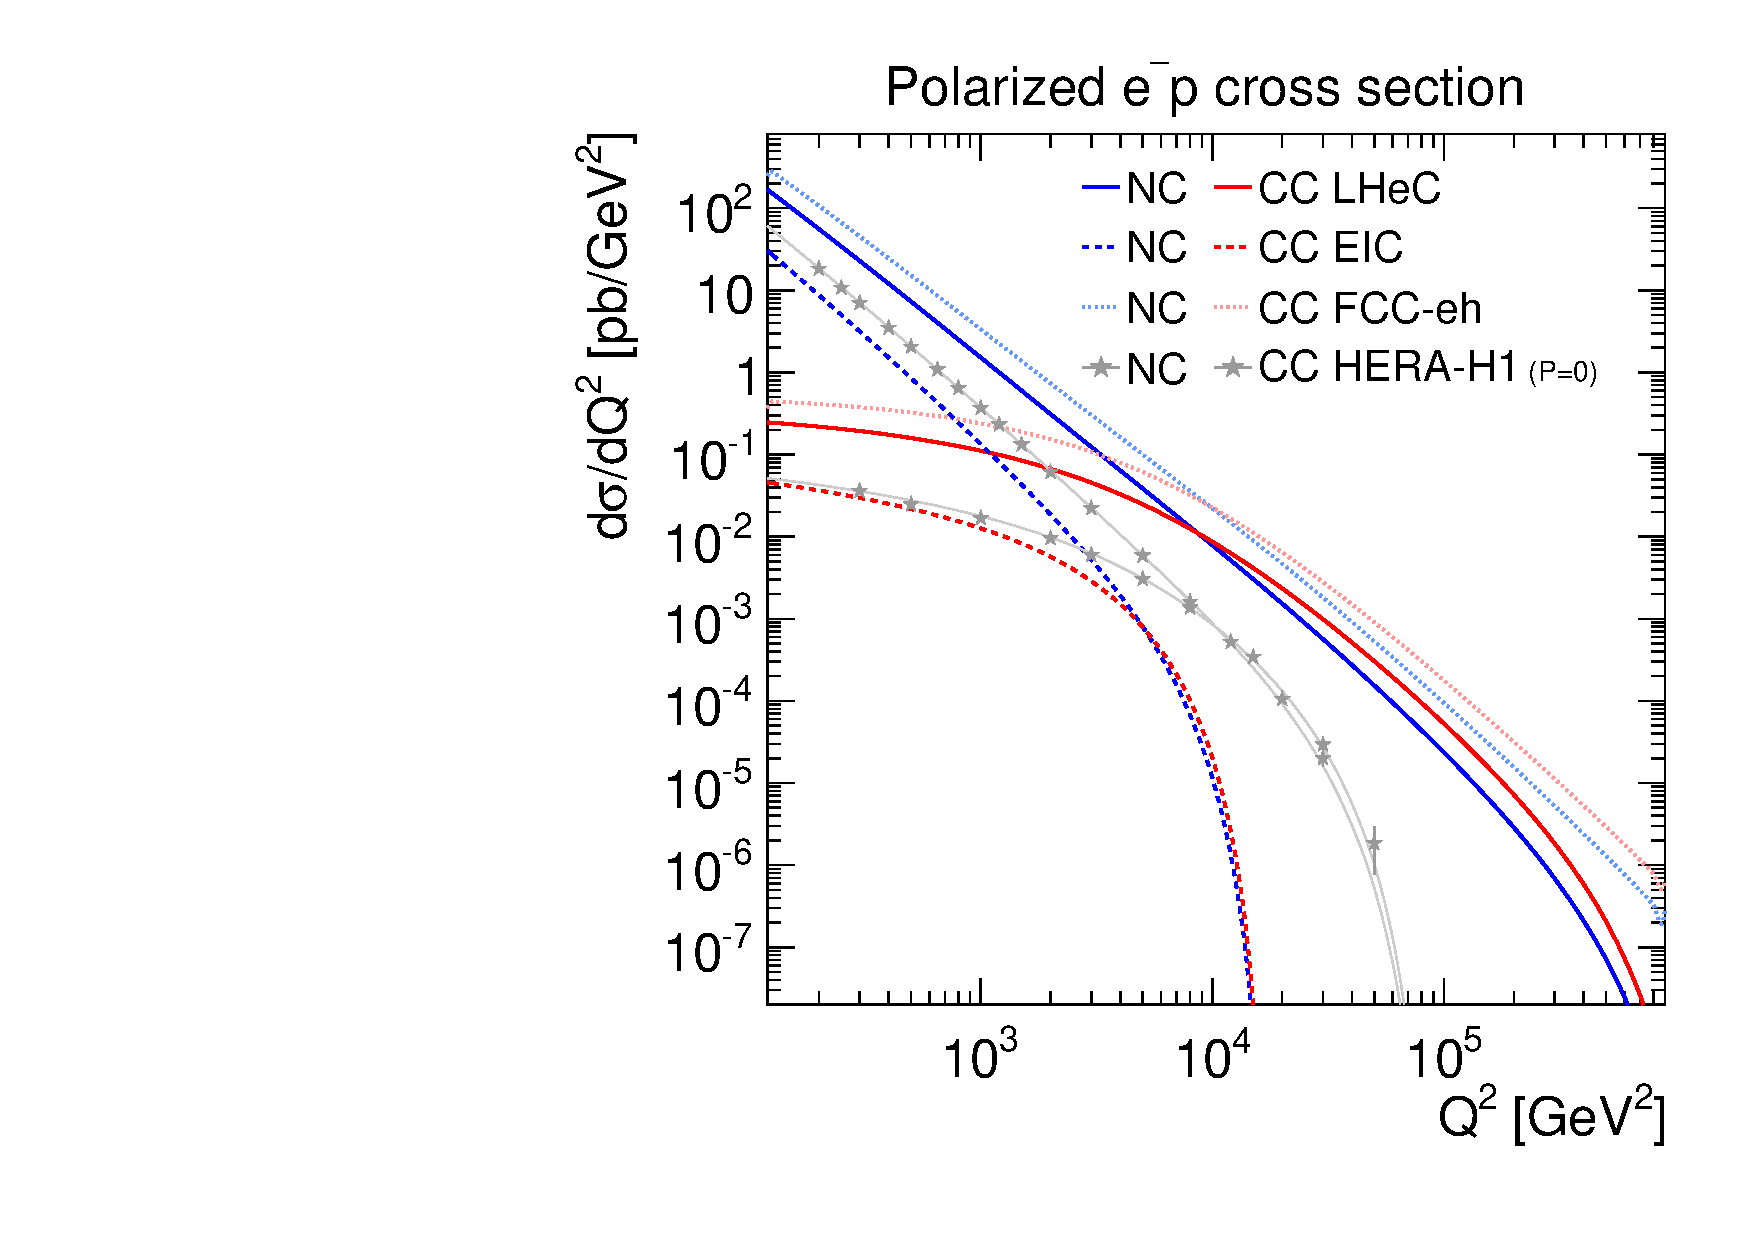
\includegraphics[width=0.52\textwidth]{plot_GraphsDsigmaDQ2_FCCEIC_opt}
  \caption{{Single differential inclusive DIS cross sections for
      $e^-p$ NC  and CC DIS at the
      EIC, HERA, LHeC and FCC-eh.
%      LHeC for two different electron beam energies
%      ($E_e=50\,\GeV$ and 60\,\GeV).
%      Cross sections for longitudinal
%      electron beam
%      polarisations of $P_e=-0.8$ and $+0.8$ are displayed.
%      For comparison also measurements at center-of-mass energies
%      of $\sqrt{s}=920$ by H1 at HERA for unpolarised ($P=0\,\%$)
%      electron beams are displayed.
  }}
  \label{fig:dSigmaFacilities}
\end{figure}

{\color{green}Two alternative versions of this plot are below}
\begin{figure}[h!b]
  \centering
  \includegraphics[width=0.38\textwidth]{plot_GraphsDsigmaDQ2_LHeC_opt}
  \hskip0.05\textwidth
  \includegraphics[width=0.38\textwidth]{plot_GraphsDsigmaDQ2_FCC_opt}
  \caption{
    Left: Inclusive NC and CC DIS cross sections as a function of \Qsq
    for two different polarisation states $P=\pm0.8$ and for two different electron
    beam energies, $E_e=50$ and $60\,\GeV$.
    For comparison, also the HERA measurements are displayed for $P=0$.
    Right: Inclusive NC and CC DIS cross sections as a function of
    \Qsq for different proton beam energies, $E_p=7$, 20 and
    50\,TeV. The latter two are possible at the future FCC.
    {\color{red} Appendix/additional figure?}
tfa  }
  \label{fig:dSigmaopt}
\end{figure}

%--------------------------------------------------------------------
%                            Summary
%--------------------------------------------------------------------
\clearpage
\section{Summary and Conclusion}
\label{sect:Conclusion}
{\color{green} Text partially equivalent to the FCC-CDR}
%
Simulated neutral current and charged current inclusive DIS cross
sections at the LHeC are explored for a determination of the
fundamental parameters of electroweak theory and for precision tests
of the Standard Model formalism.
%
The high center-of-mass energy and the large integrated
luminosity at the LHeC will allow for the first time precision electroweak
measurement in DIS at high scales.
%


Highest precision is achieved for the measurement of the $W$-boson
mass with a prospected experimental uncertainty of up to
$\Delta\mW=5\,\MeV$, and an outstanding  
precision can also be achieved for the weak neutral current couplings of
light quarks to the $Z$ boson.
%
The space-like momentum transfer in DIS further allows for unique
scale dependent test of the electroweak theory, both, for neutral and
charged currents.
This includes for instance scale dependent measurements of the effective
weak mixing angle in the range of about $40<\sqrt{\Qsq}<700\,\GeV$
with a precision up to a few permille.

Further direct measurements, as for instance Higgs production,
top-quark production or single $W$ or $Z$
production cross sections, or vector-boson-scattering cross sections,
as well as heavy flavor cross sections in NC and CC DIS, will provide further
improvements for electroweak precision measurements.

The measurements will not be limited by the need for parton
distribution functions.
In many cases, the measurements are complementary to measurements in
$e^+e^-$ or hadron-hadron collisions.


In summary, the inclusive NC and CC DIS cross sections measured at
LHeC provide a unique opportunity to perform high-precision
determinations of fundamental electroweak parameters and test the
quantum  nature of electroweak processes with high precision.
Complementarity!

Unique measurements will be made for weak charged currents and
for the scale-dependence of electroweak interactions.

{\color{red}We studied in a traditional way NC and CC separately.
Many models predict changes to NC and CC simultaneously. A such, a
simultaneous determination of NC and CC observables is reasonable}



%--------------------------------------------------------------------
%  Optional material, to be discussed...
%--------------------------------------------------------------------
\clearpage
\section{Optional material}
\subsection{Electron couplings}
{\color{magenta} Todo: Discussion about \ve\ and \gae.}
\begin{figure}[htbp]
    \centering
    \includegraphics[width=0.40\textwidth]{plot_couplings_e}
  \caption{
    Weak-neutral-current vector and axial-vector couplings of the electron
    at 68\,\% confidence level~(C.L.) for
    simulated LHeC data with $E_e=60\,\GeV$.
    The LHeC expectations are compared with results from the combined
    analysis of LEP+SLD data~\cite{ALEPH:2005ab}, which are much more precise.
    {\color{red}We need to re-do this plot, but I don't know if it is
      at all reasonable to show it...}
  }
  \label{fig:couplings2}
\end{figure}


%-------------------------------------------------------------------- 
\clearpage
\subsection{Other $\sin^2\theta_\text{W}^{\text{eff},\ell}(\mz^2)$ or $\kappa^\prime$ fits}
Results from  more specific fits of
$\sin^2\theta_\text{W}^{\text{eff},\ell}(\mz^2)$.

\begin{table}[htb]
  \centering
  \small
  %\begin{tabular}{lr@{\hskip4pt}lccc}
  \begin{tabular}{lcccccc}
    \toprule
    Fit parameters &  Parameter & SM & \multicolumn{4}{c}{Expected uncertainties} \\
    \cmidrule(lr){4-7}
    &   of interest  &  value    & LHeC-50 & LHeC-60 & LHeC-50 & LHeC-60 \\
    &                &          &  \multicolumn{2}{c}{\footnotesize{($\delta_\text{uncor.}=0.50\,\%$)}} & \multicolumn{2}{c}{\footnotesize{($\delta_\text{uncor.}=0.25\,\%$)}} \\
    \midrule
    $\kappa^\prime_{\text{NC},f}$, PDFs
    & $\sin^2\theta_\text{W}^{\text{eff},\ell}(\mz^2)$ & 0.23154 & $0.00033$ & $0.00025$ & 0.00022 & $0.00015$ \\ % ok
    $\kappa^\prime_{\text{NC},f}$, $\rho^\prime_{\text{NC},f}$, PDFs
    & $\sin^2\theta_\text{W}^{\text{eff},\ell}(\mz^2)$ & 0.23154 & 0.00071  & 0.00036 &  0.00056 & 0.00023 \\ %ok
    $\kappa^\prime_{\text{NC},e}$, PDFs
    &  $\sin^2\theta_\text{W}^{\text{eff},e}(\mz^2)$   & 0.23154 & $0.00059$  & $0.00047$ & 0.00038 & $0.00028$ \\
    $\kappa^\prime_{\text{NC},e}$, $\kappa^\prime_{\text{NC},u}$, $\kappa^\prime_{\text{NC},d}$, PDFs
    &  $\sin^2\theta_\text{W}^{\text{eff},e}(\mz^2)$   & 0.23154 & 0.00111 & 0.00095 & 0.00069 & 0.00056\\ %ok
%    \midrule
    $\kappa^\prime_{\text{NC},f}$
    & $\sin^2\theta_\text{W}^{\text{eff},\ell}(\mz^2)$ & 0.23154 & 0.00028 & 0.00023 & 0.00017 & 0.00014 \\ % ok
    \bottomrule
    % kappa' fit with PDFs:
    %  0.00033 & 0.00025 & 0.00022 & 0.00015
    % kappa' fit without PDFs:
    %  0.00028 & 0.00023 & 0.00017 & 0.00014
    %    $\sin^2\theta_\text{W}^{\text{eff},\ell}$ (PDG)      & $0.23148$    & $\pm0.00013$    \\
    %    $\sin^2\theta_\text{W}^{\text{eff},\ell}$ (LEP+SLD)  & $0.23154$    & $\pm0.00016$    \\
    %    $\sin^2\theta_\text{W}^{\text{eff},\ell}$ (Tevatron) & $0.23148$    & $\pm0.00033$    \\
    %    $\sin^2\theta_\text{W}^{\text{eff},\ell}$ (LHC)      & $0.23131$    & $\pm0.00033$    \\
    %    $\sin^2\theta_\text{W}^{\text{eff},\ell}$ ($A_{fb}^{0,\ell}$ LEP)  & $0.23099$    & $\pm0.00053$    \\
%\hline
  \end{tabular}
  \caption{
    Determination of $\sin^2\theta_\text{W}^{\text{eff},\ell}(\mz^2)$
    with inclusive DIS data at the LHeC for different scenarios.
    Since the value of the effective weak mixing angle at the $Z$ pole
    cannot be determined directly in DIS, a fit of the
    $\kappa^\prime_{\text{NC},f}$ parameter is performed instead and
    its uncertainty is translated to
    $\sin^2\theta_\text{W}^{\text{eff},\ell}(\mz^2)$.
    Different assumptions on the fit parameters are studied, and
    results include uncertainties from the PDFs.
    Only the last line shows results where the PDF parameters are kept fixed.
    See text for more details.
    {\color{red}Not yet referenced and discussed in the text.}
  }
  \label{tab:sweff}
\end{table}



%-------------------------------------------------------------------- 
\clearpage
\subsection{Best uncertainties for $\rho^\prime$ and $\kappa^\prime$
  parameters}
In a fit of a single anomalous form factor, we obtain following uncertainties. 
{\color{blue} Maximum sensitivity is obtained in 1-parameter fits, and prospects are collected in table:~\ref{tab:rhopwithcorrelations}.}
\begin{table}[bhtp]
  \footnotesize
  \centering
  \begin{tabular}{lcr@{$\,\pm\,$}lr@{$\,\pm\,$}l}
    \hline
    Fit parameters & Parameter & \multicolumn{2}{c}{LHeC}& \multicolumn{2}{c}{FCC}  \\
    \hline
    \rhopu+PDF & \rhopu &  1  &  0.009    & 1  & 0.004  \\
    \kappu+PDF & \kappu &  1  &  0.004    & 1  & 0.003  \\
    \rhopd+PDF & \rhopd &  1  &  0.014    & 1  & 0.006  \\
    \kappd+PDF & \kappd &  1  &  0.023    & 1  & 0.013  \\
    \rhope+PDF & \rhope &  1  &  0.006    & 1  & 0.003  \\
    \kappe+PDF & \kappe &  1  &  0.003    & 1  & 0.002  \\
    \hline
    \rhopq+PDF & \rhopq &  1  &  0.0059    & 1  & 0.0027  \\
    \kappq+PDF & \kappq &  1  &  0.0038    & 1  & 0.0024  \\
    \hline
    \rhopf+PDF & \rhopf &  1  &  0.0031    & 1  & 0.0015  \\ %0.00145641
    \kappf+PDF & \kappf &  1  &  0.0019    & 1  & 0.0011  \\
    \hline
    \\
    \multicolumn{3}{l}{Expectations for \rhopW{,f} (CC)} \\
    \hline
    % log.final.PAR19eq50.3p.PDF.2.txt
    \rhopW{,f}+PDF   & \rhopW{,f}                &  1  &   0.0043  & 1  & 0.0027 \\
    \rhopW{,eq}+PDF  & \rhopW{,eq}               &  1  &   0.0027  & 1  &  0.0011\\
    \rhopW{,e\bar{q}}+PDF  & \rhopW{,e\bar{q}}   &  1  &   0.0030  & 1  &  0.0012\\
    \hline
  \end{tabular}
  \caption{
    {\color{red} note: these numbers need to be updated, if we want to
    include such a table.}
    Results for $\rhop{}$, $\kapp{}$ and \rhopW{} parameters.
  }
  \label{tab:rhopwithcorrelations}
\end{table}




%-------------------------------------------------------------------- 
\clearpage
\subsection{Polarisation asymmetry in NC, and polarisation in CC}
{\color{green}A potential additional plot could be about the
  polarisation asymmetry, but this maybe opens a long discussion...}
\begin{figure}[h!b]
\begin{center}
   \includegraphics[width=0.40\textwidth]{{figures/fcc_asymmetry}.pdf}
   \hskip1cm
   \includegraphics[width=0.40\textwidth]{{figures/fcc_CCtot}.pdf}
\end{center}
\caption{
  Left: Neutral-current polarisation asymmetry as a function of
  \Qsq\ integrated over $x$ for FCC-eh simulated data. The polarisation asymmetry
  is displayed for pure photon exchange, which is zero
  by definition, % due to the absence of parity violating terms.
  for calculations including only the interference terms $\gamma^*Z$,
  and for predictions including also purely weak effects, $ZZ$.
  The full circles illustrate simulated data points, which have
  uncertainties invisible at the chose scales.
  Right: Charged-current cross sections measured with different lepton
  polarisation states and for electron (red) and positron
  (blue) beams. The full circles illustrate FCC-eh simulated data,
  whereas the open circles show H1 measurements. The data are scaled
  by the the center-of-mass energies of the respective collider.
  The error bars are smaller than the markers.
}
\label{fig:crosssections}
\end{figure}


%--------------------------------------------------------------------
%                          Acknowledgements
%--------------------------------------------------------------------
\clearpage
\section*{Acknowledgements}
Acknowledgements: A.~Sch\"oning, M.~Klein, S.~Schmitt



%--------------------------------------------------------------------
%\input{fcc_draft}


%--------------------------------------------------------------------
%   Results from LHeC inclusive DIS data
%--------------------------------------------------------------------
\clearpage
\section{Tables}
\subsection{Determinations of single parameters}
\begin{table}[h]
  \footnotesize
  \centering
  \begin{tabular}{lcr@{$\,\pm\,$}lr@{$\,\pm\,$}l}
    \hline
    Fit parameters & Parameter & \multicolumn{2}{c}{LHeC}& \multicolumn{2}{c}{FCC}  \\
    \hline
    % log.fcc.6p.u.d.e.txt
    % EPRC.rhopu                =            1   +/-   0.00864794
    % EPRC.zkapu                =            1   +/-   0.00886882
    % EPRC.rhopd                =            1   +/-   0.028591
    % EPRC.zkapd                =            1   +/-   0.0438381
    % EPRC.rhope                =            1   +/-   0.0136914
    % EPRC.zkape                =            1   +/-   0.00510635
    \rhopd+\kappd+\rhopu+\kappu+\rhop{,e}+\kapp{,e}+PDF
    & \rhopu &  1  &  0.031    & 1  & 0.009 \\
    & \kappu &  1  &  0.013    & 1  & 0.009 \\
    & \rhopd &  1  &  0.062    & 1  & 0.029   \\
    & \kappd &  1  &  0.076    & 1  & 0.044  \\
    & \rhope &  1  &  0.036    & 1  & 0.014  \\
    & \kappe &  1  &  0.008    & 1  & 0.005 \\
    \hline
    % /nfs/dust/h1/group/britzger/alpos/Alpos/../log.fcc.4p.u.d.txt
    % EPRC.rhopu                =            1   +/-   0.00748481
    % EPRC.zkapu                =            1   +/-   0.00663437
    % EPRC.rhopd                =            1   +/-   0.0159018
    % EPRC.zkapd                =            1   +/-   0.0419873
    %lhec
    % EPRC.rhopu                =            1   +/-   0.0185425
    % EPRC.zkapu                =            1   +/-   0.0102184
    % EPRC.rhopd                =            1   +/-   0.0394555
    % EPRC.zkapd                =            1   +/-   0.0757502
    \rhopd+\kappd+\rhopu+\kappu+PDF
    & \rhopu &  1  &  0.019  & 1  & 0.007   \\
    & \kappu &  1  &  0.010  & 1  & 0.007   \\
    & \rhopd &  1  &  0.039  & 1  & 0.016   \\
    & \kappd &  1  &  0.076  & 1  & 0.042   \\
    \hline
    % /nfs/dust/h1/group/britzger/alpos/Alpos/../log.fcc.4p.e.q.txt
    %rhopq                     =            1   +/-   0.00827489
    %zkapq                     =            1   +/-   0.005199
    %EPRC.rhope                =            1   +/-   0.0100664
    %EPRC.zkape                =            1   +/-   0.00504328
    \rhop{,q}+\kapp{,q}+\rhop{,e}+\kapp{,e}+PDF
    & \rhop{,q} & 1 &  0.029  & 1 &  0.008  \\
    & \kapp{,q} & 1 &  0.007  & 1 &  0.005 \\
    & \rhop{,e} & 1 &  0.032  & 1 &  0.010 \\
    & \kapp{,e} & 1 &  0.008  & 1 &  0.005 \\
    \hline
    % /nfs/dust/h1/group/britzger/alpos/Alpos/../log.fcc.4p.e.q.txt
    %rhopq                     =            1   +/-   0.00827489
    %zkapq                     =            1   +/-   0.005199
    %EPRC.rhope                =            1   +/-   0.0100664
    %EPRC.zkape                =            1   +/-   0.00504328
    \rhop{,q}+\kapp{,q}+\rhop{,e}+\kapp{,e}+PDF
    & \rhop{,q} & 1 &  0.029  & 1 &  0.008  \\
    & \kapp{,q} & 1 &  0.007  & 1 &  0.005 \\
    & \rhop{,e} & 1 &  0.032  & 1 &  0.010 \\
    & \kapp{,e} & 1 &  0.008  & 1 &  0.005 \\
    \hline
    % /nfs/dust/h1/group/britzger/alpos/Alpos/
    \rhopu+\kappu+PDF
    & \rhopu &  1  &  0.011    & 1 & 0.005\\
    & \kappu &  1  &  0.005    & 1 & 0.003\\
    \hline
    % /nfs/dust/h1/group/britzger/alpos/Alpos/
    \rhopd+\kappd+PDF
    & \rhopd &  1  &  0.022    &  1  & 0.011 \\
    & \kappd &  1  &  0.038    &  1  & 0.021 \\
    \hline
    \rhop{,e}+\kapp{,e}+PDF
    & \rhope &  1  & 0.009      & 1  & 0.005 \\
    & \kappe &  1  & 0.005      & 1  & 0.003  \\
    \hline
    \rhop{,f}+\kapp{,f}+PDF
    & \rhope &  1  & 0.0042      & 1  & 0.0022 \\
    & \kappe &  1  & 0.0026      & 1  & 0.0016  \\
    \hline
    \\
    \multicolumn{3}{l}{Fits including \rhopW{,f} (CC)} \\
    \hline
    % log.final.PAR19eq50.3p.PDF.2.txt
    \rhop{,f}$+$\kapp{,f}$+$\rhopW{,f}+PDF
    & \rhop{f}   &  1  &  0.0045   & 1  & 0.0021 \\
    & \kapp{f}   &  1  &  0.0027   & 1  & 0.0015 \\
    & \rhopW{,f} &  1  &  0.0043   & 1  & 0.0027 \\
    % & $\rhop{W,f}=1.002\pm0.008$ & \\
    \hline
  \end{tabular}
  \caption{
    Results for $\rhop{}$, $\kapp{}$ and \rhopW{} parameters, and their
    correlation coefficients.
  }
  \label{tab:rhopwithcorrelations}
\end{table}


\begin{table}[h]
  \footnotesize
  \centering
  \begin{tabular}{lr@{$\,=\,$}c@{$\,\pm\,$}l|cccccc}
    \hline
    Fit parameters & \multicolumn{3}{c}{Result} & \multicolumn{6}{l}{Correlation} \\
    \hline
    % /nfs/dust/h1/group/britzger/alpos/Alpos/
    \rhopd+\kappd+\rhopu+\kappu+\rhop{,e}+\kapp{,e}+PDF
    & \rhopu &    &      & 1.00 \\
    & \kappu &    &      & 0.  & 1.00 \\
    & \rhopd &    &      &$    $& $   $ & 1.00 \\
    & \kappd &    &      &$    $& $   $ &  & 1.00 \\
    & \rhope &    &      &      &       &  &      &  1.00 \\
    & \kappe &    &      & 0.   &       &  &      &  & 1.00 \\
    \hline
    % /nfs/dust/h1/group/britzger/alpos/Alpos/
    \rhopd+\kappd+\rhopu+\kappu+PDF
    & \rhopu &    &      & 1.00 \\
    & \kappu &    &      & 0.  & 1.00 \\
    & \rhopd &    &      &$    $& $   $ & 1.00 \\
    & \kappd &    &      &$    $& $   $ &  & 1.00 \\
    \hline
    % /nfs/dust/h1/group/britzger/alpos/Alpos/
    \rhop{,q}+\kapp{,q}+\rhop{,e}+\kapp{,e}+PDF
    & \rhop{,e} &    &     & 1.00 \\
    & \kapp{,e} &    &     & 0.  & 1.00 \\
    & \rhop{,q} &    &     &     & 0.  & 1.00 \\
    & \kapp{,q} &    &     & 0.  & $0$ & 0.0  & 1.00 \\
    \hline
    % /nfs/dust/h1/group/britzger/alpos/Alpos/
    \rhopu+\kappu+PDF
    & \rhopu &    &      & 1.00 \\
    & \kappu &    &      & 0.  & 1.00 \\
    \hline
    % /nfs/dust/h1/group/britzger/alpos/Alpos/
    \rhopd+\kappd+PDF
    & \rhopd &    &      & 1.00 \\
    & \kappd &    &      &  & 1.00 \\
    \hline
    % /nfs/dust/h1/group/britzger/alpos/Alpos/
    \rhop{,e}+\kapp{,e}+PDF
    & \rhope &    &      &  1.00 \\
    & \kappe &    &      &  & 1.00 \\
    \hline
    \\
    \multicolumn{3}{l}{Fits including \rhopW{,f} (CC)} \\
    \hline
    % log.final.PAR19eq50.3p.PDF.2.txt
    \rhop{,f}$+$\kapp{,f}$+$\rhopW{,f}+PDF
    & \rhop{f}   &    &     & 1.00 & \\
    & \kapp{f}   &    &     & 0. & 1.00  \\
    & \rhopW{,f} &    &     & 0. & $0.$ & 1.00\\
    % & $\rhop{W,f}=1.002\pm0.008$ & \\
    \hline
  \end{tabular}
  \caption{
    Results for $\rhop{}$, $\kapp{}$ and \rhopW{} parameters, and their
    correlation coefficients.
  }
  \label{tab:rhopwithcorrelations}
\end{table}


% ------------------------------------------------------------------------
%
% ------------------------------------------------------------------------
\clearpage
\section*{Useless stuff}
%Reasonable examples are determinations of (all) the weak neutral current
%couplings, $g_A^{f}$ and $g_V^{f}$ with $f=(e,u,d,s,c,b,t)$,
%or more general, directly the $\rho_{\text{NC}, f}$ and
%$\kappa_{\text{NC}, f}$ parameters.
These can be done either in the scale-indpendent LO approximation, by
taking the scale-dependent loop corrections from theory, or their
effective values can be determined at different scales.
More commonly though, the effective weak mixing
angle $\sin\theta_{\text{W}}^{\text{eff},f}:=\kappa_{\text{NC}, q/e}\ \sw$
is tested at different scales, while also this quantity has an
important scheme dependent component (see Ref.~\ref{pdg18} for a
concise dicsussion).
Noteworthy, most of the precision measurements are performed in the
time-like domain, i.e.\ for $\mu^2>0$, whereas DIS is mediated by space-like
momentum transfer, $\Qsq=-q^2$, and thus $q^2<0$.
In DIS at the LHeC, in addition, a large kinematic range can be tested.

Complementary, the measurement of the weak boson masses yields an interesting testing
case of the theory, in particular the measurement of \mw.
This is because \mw\ can be considered as input parameter to the
formalism, or alternatively, if the precision measurement of \gf\ is
been taken as input~\cite{Tishchenko:2012ie}, then \mw becomes a
prediction and can be confronted with the measurement directly.
